\documentclass[aspectratio=169, 11pt]{beamer}
\usetheme{Madrid}
\usecolortheme{whale}
\setbeamercolor{frametitle}{bg=blue!8, fg=black}
\setbeamercolor{title}{bg=blue!12, fg=black}
\setbeamercolor{structure}{fg=blue!50!black}
\setbeamercolor{item}{fg=blue!50!black}
\setbeamertemplate{navigation symbols}{}
\setbeamertemplate{footline}{
  \leavevmode\hbox{%
    \begin{beamercolorbox}[wd=.35\paperwidth,ht=2.5ex,dp=1ex,left]{author in head/foot}%
      \hspace*{1em}\footnotesize Machine Learning with R (Dr.\ Endri Ra\c{c}o)
    \end{beamercolorbox}%
    \begin{beamercolorbox}[wd=.35\paperwidth,ht=2.5ex,dp=1ex,center]{title in head/foot}%
      \footnotesize Regularization
    \end{beamercolorbox}%
    \begin{beamercolorbox}[wd=.3\paperwidth,ht=2.5ex,dp=1ex,right]{date in head/foot}%
      \footnotesize Week 4, 2025 \hspace*{1em} \insertframenumber{} / \inserttotalframenumber \hspace*{1em}
    \end{beamercolorbox}}%
}
\usepackage{amsmath,amssymb,mathtools}
\usepackage{tikz}
\usetikzlibrary{arrows.meta, positioning, calc, shapes, decorations.pathreplacing, patterns}
\usepackage{pgfplots}
\pgfplotsset{compat=1.18}
\usepackage{booktabs}
\usepackage{xcolor}
\definecolor{accent}{RGB}{59,130,246}
\definecolor{darkblue}{RGB}{30,39,97}
\definecolor{softred}{RGB}{239,68,68}
\definecolor{softgreen}{RGB}{16,185,129}
\definecolor{amber}{RGB}{245,158,11}
\definecolor{muted}{RGB}{100,116,139}
\definecolor{orange}{RGB}{249,115,22}
\definecolor{beige}{RGB}{245,235,210}
\title{Linear Model Selection \& Regularization}
\subtitle{Subset Selection, Ridge Regression \& Lasso --- ISLR Chapter 6}
\author{Machine Learning with R}
\institute{Dr.\ Endri Ra\c{c}o}
\date{Week 4, 2025}
\begin{document}
\begin{frame}\titlepage\end{frame}

\begin{frame}{The Problem: Too Many Predictors}
\begin{columns}
\column{0.55\textwidth}
\textbf{Weeks 1--3:} OLS with all $p$ predictors

\textbf{Problem:} What if $p$ is large?
\begin{itemize}
  \item Overfitting (low bias, high variance)
  \item Collinearity (unstable $\hat{\beta}$)
  \item $p > n$: OLS doesn't even work!
  \item Interpretation: which variables matter?
\end{itemize}
\vspace{0.3em}
\textbf{Three strategies:}
\begin{enumerate}
  \item Subset selection
  \item Shrinkage (Ridge, Lasso)
  \item Dimension reduction (PCR, PLS)
\end{enumerate}
\column{0.4\textwidth}
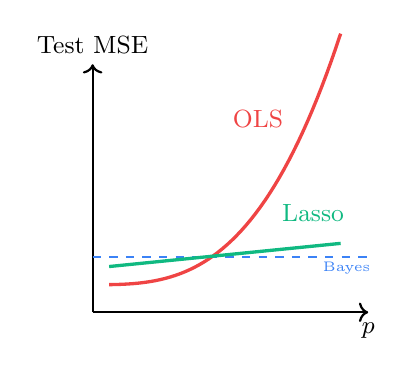
\begin{tikzpicture}[scale=0.7]
  \draw[->, thick] (0,0) -- (5,0) node[below] {\small $p$};
  \draw[->, thick] (0,0) -- (0,4.5) node[above] {\small Test MSE};
  \draw[softred, very thick, domain=0.3:4.5, samples=50] plot (\x, {0.5 + 0.05*\x*\x*\x});
  \draw[accent, thick, dashed] (0, 1) -- (5, 1);
  \node[accent, right] at (4, 0.8) {\tiny Bayes};
  \node[softred] at (3, 3.5) {\small OLS};
  \draw[softgreen, very thick, domain=0.3:4.5, samples=50] plot (\x, {0.8 + 0.1*\x});
  \node[softgreen] at (4, 1.8) {\small Lasso};
\end{tikzpicture}
\end{columns}
\end{frame}

\begin{frame}{Today's Roadmap}
\begin{columns}
\column{0.48\textwidth}
\begin{enumerate}
  \item Best subset selection
  \item Forward/backward stepwise
  \item Ridge regression
  \item The Lasso
  \item Elastic Net
  \item Choosing $\lambda$ via CV
  \item PCR and PLS (preview)
\end{enumerate}
\column{0.48\textwidth}
\textbf{Dataset:} \texttt{Hitters}

$n = 263$ baseball players

$p = 19$ predictors

$Y =$ Salary (thousands \$)

\vspace{0.5em}
\textbf{Key question:}

Which stats predict salary?

Can we build a \textbf{sparse}, interpretable model?
\end{columns}
\end{frame}

\begin{frame}{The Hitters Dataset}
\begin{columns}
\column{0.5\textwidth}
\textbf{263 MLB players, 19 predictors:}
\begin{itemize}
  \item AtBat, Hits, HmRun, Runs, RBI
  \item Walks, Years, CAtBat, CHits
  \item CHmRun, CRuns, CRBI, CWalks
  \item League, Division, PutOuts
  \item Assists, Errors, NewLeague
\end{itemize}
\vspace{0.3em}
59 players have missing Salary $\Rightarrow$ drop them ($n = 263$)
\column{0.45\textwidth}
\textbf{Challenge:}
\begin{itemize}
  \item Many predictors are correlated (career stats $\approx$ rescaled season stats)
  \item Which subset matters?
  \item OLS uses all 19 $\Rightarrow$ overfitting risk
\end{itemize}
\vspace{0.3em}
\footnotesize R: \texttt{Hitters <- na.omit(Hitters)}
\end{columns}
\end{frame}

% ════════════ SUBSET SELECTION ════════════
\begin{frame}{Best Subset Selection}
\begin{columns}
\column{0.55\textwidth}
\textbf{Idea:} Fit all $2^p$ possible models, pick the best

\textbf{Algorithm:}
\begin{enumerate}
  \item For each $k = 0, 1, \ldots, p$:
  \begin{itemize}
    \item Fit all $\binom{p}{k}$ models with $k$ predictors
    \item Keep the one with smallest RSS
  \end{itemize}
  \item Among the $p+1$ ``best'' models, select using CV, $C_p$, BIC, or Adj.~$R^2$
\end{enumerate}
\column{0.4\textwidth}
\textbf{Problem: Combinatorial explosion}
\begin{tabular}{cc}
\toprule
$p$ & \# Models \\
\midrule
5 & 32 \\
10 & 1,024 \\
20 & \textcolor{softred}{1,048,576} \\
30 & \textcolor{softred}{$10^9$} \\
\bottomrule
\end{tabular}
\vspace{0.3em}
\textcolor{softred}{Infeasible for $p > 40$!}

\footnotesize R: \texttt{leaps::regsubsets()}
\end{columns}
\end{frame}

\begin{frame}{Stepwise Selection: A Practical Alternative}
\begin{columns}
\column{0.48\textwidth}
\textbf{Forward stepwise:}
\begin{enumerate}
  \item Start with null model ($k=0$)
  \item Add the predictor that most improves fit
  \item Repeat until $k = p$
  \item Select best via CV/BIC/$C_p$
\end{enumerate}
Fits $1 + p(p+1)/2$ models

\column{0.48\textwidth}
\textbf{Backward stepwise:}
\begin{enumerate}
  \item Start with full model ($k=p$)
  \item Remove the least useful predictor
  \item Repeat until $k = 0$
  \item Select best via CV/BIC/$C_p$
\end{enumerate}
Requires $n > p$ (so OLS works)
\end{columns}
\vspace{0.5em}
\centering
\begin{tabular}{lcc}
\toprule
Method & \# Models fitted & Works if $p > n$? \\
\midrule
Best subset & $2^p$ & No \\
Forward & $1 + p(p+1)/2$ & \textcolor{softgreen}{Yes} \\
Backward & $1 + p(p+1)/2$ & No \\
\bottomrule
\end{tabular}
\end{frame}

\begin{frame}{Choosing the Best Model: $C_p$, BIC, Adj.~$R^2$}
\begin{columns}
\column{0.48\textwidth}
\textbf{Mallow's $C_p$:}
$$C_p = \frac{1}{n}(\text{RSS} + 2d\hat{\sigma}^2)$$
Penalizes complexity ($d$ = \# predictors)

\vspace{0.3em}
\textbf{BIC:}
$$\text{BIC} = \frac{1}{n}(\text{RSS} + \log(n) \cdot d \hat{\sigma}^2)$$
Heavier penalty $\Rightarrow$ sparser models

\column{0.48\textwidth}
\textbf{Adjusted $R^2$:}
$$\text{Adj.\ } R^2 = 1 - \frac{\text{RSS}/(n-d-1)}{\text{TSS}/(n-1)}$$
Penalizes for adding useless predictors

\vspace{0.5em}
\textbf{Best approach:}

\textcolor{accent}{Cross-validation} (Week 3)

Direct estimate of test error

No formula-based approximation needed
\end{columns}
\end{frame}

\begin{frame}{Subset Selection on Hitters}
\begin{columns}
\column{0.5\textwidth}
\textbf{Best subset results:}
\begin{tabular}{ccc}
\toprule
$d$ & RSS & BIC \\
\midrule
1 & 36,180 & $-90$ \\
2 & 33,420 & $-128$ \\
3 & 32,110 & $-138$ \\
\textcolor{softgreen}{6} & \textcolor{softgreen}{29,850} & \textcolor{softgreen}{$-148$} \\
10 & 28,940 & $-140$ \\
19 & 28,510 & $-110$ \\
\bottomrule
\end{tabular}
\vspace{0.3em}
BIC selects 6 predictors

$C_p$ selects 10

Adj.~$R^2$ selects 11
\column{0.45\textwidth}
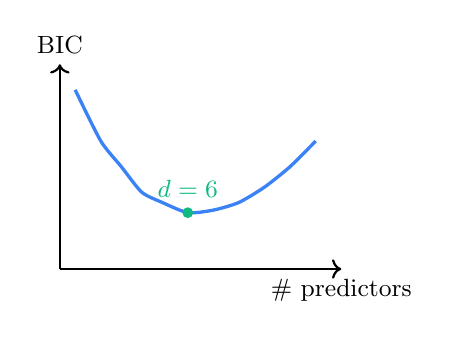
\begin{tikzpicture}[scale=0.65]
  \draw[->, thick] (0,0) -- (5.5,0) node[below] {\small \# predictors};
  \draw[->, thick] (0,0) -- (0,4) node[above] {\small BIC};
  \draw[accent, very thick, smooth, tension=0.4] plot coordinates {(0.3,3.5)(0.8,2.5)(1.2,2.0)(1.6,1.5)(2,1.3)(2.5,1.1)(3,1.15)(3.5,1.3)(4,1.6)(4.5,2.0)(5,2.5)};
  \fill[softgreen] (2.5, 1.1) circle (3pt);
  \node[softgreen, above] at (2.5, 1.2) {\small $d=6$};
\end{tikzpicture}
\vspace{0.3em}
\textit{BIC penalizes more $\Rightarrow$ sparser model}
\end{columns}
\end{frame}

% ════════════ RIDGE REGRESSION ════════════
\begin{frame}{Ridge Regression: The Idea}
\textbf{OLS minimizes:} $\text{RSS} = \sum_{i=1}^n (y_i - \hat{y}_i)^2$

\textbf{Ridge minimizes:} $\text{RSS} + \lambda \sum_{j=1}^p \beta_j^2$

\vspace{0.5em}
\begin{columns}
\column{0.5\textwidth}
$$\hat{\beta}^R_\lambda = \arg\min_\beta \left\{ \text{RSS} + \lambda \sum_{j=1}^p \beta_j^2 \right\}$$
\begin{itemize}
  \item $\lambda \geq 0$ is the \textbf{tuning parameter}
  \item $\lambda = 0$: identical to OLS
  \item $\lambda \to \infty$: all $\hat{\beta}_j \to 0$
  \item $\lambda$ controls the bias-variance trade-off
\end{itemize}
\column{0.45\textwidth}
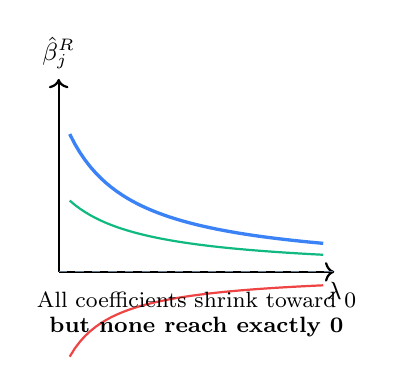
\begin{tikzpicture}[scale=0.7]
  \draw[->, thick] (0,0) -- (5,0) node[below] {\small $\lambda$};
  \draw[->, thick] (0,0) -- (0,3.5) node[above] {\small $\hat{\beta}_j^R$};
  \draw[accent, very thick, domain=0.2:4.8, samples=50] plot (\x, {3/(1+\x)});
  \draw[softred, thick, domain=0.2:4.8, samples=50] plot (\x, {-2/(1+1.5*\x)});
  \draw[softgreen, thick, domain=0.2:4.8, samples=50] plot (\x, {1.5/(1+0.8*\x)});
  \draw[muted, dashed] (0, 0) -- (5, 0);
  \node[font=\footnotesize] at (2.5, -0.5) {All coefficients shrink toward 0};
  \node[font=\footnotesize] at (2.5, -1.0) {\textbf{but none reach exactly 0}};
\end{tikzpicture}
\end{columns}
\end{frame}

\begin{frame}{Ridge: Why Shrinking Helps}
\begin{columns}
\column{0.5\textwidth}
\textbf{Bias-variance for ridge:}
$$\text{MSE} = \text{Bias}^2 + \text{Variance}$$
\begin{itemize}
  \item $\lambda \uparrow$ $\Rightarrow$ Bias $\uparrow$ (moving away from OLS)
  \item $\lambda \uparrow$ $\Rightarrow$ Variance $\downarrow$ (coefficients more stable)
  \item Optimal $\lambda$: minimizes total MSE
\end{itemize}
\vspace{0.3em}
\textbf{Especially helpful when:}
\begin{itemize}
  \item $p$ is close to or larger than $n$
  \item Predictors are correlated
  \item OLS coefficients are very large/unstable
\end{itemize}
\column{0.45\textwidth}
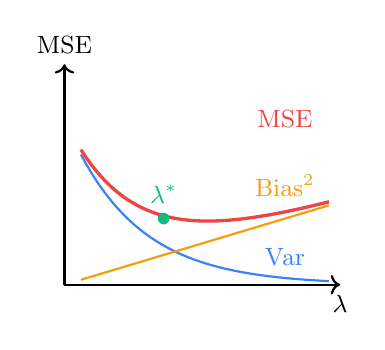
\begin{tikzpicture}[scale=0.7]
  \draw[->, thick] (0,0) -- (5,0) node[below] {\small $\lambda$};
  \draw[->, thick] (0,0) -- (0,4) node[above] {\small MSE};
  \draw[accent, thick, domain=0.3:4.8, samples=50] plot (\x, {3*exp(-0.8*\x)});
  \node[accent] at (4, 0.5) {\small Var};
  \draw[amber, thick, domain=0.3:4.8, samples=50] plot (\x, {0.3*\x});
  \node[amber] at (4, 1.8) {\small Bias$^2$};
  \draw[softred, very thick, domain=0.3:4.8, samples=50] plot (\x, {3*exp(-0.8*\x) + 0.3*\x});
  \node[softred] at (4, 3) {\small MSE};
  \fill[softgreen] (1.8, 1.2) circle (3pt);
  \node[softgreen, above] at (1.8, 1.3) {\small $\lambda^*$};
\end{tikzpicture}
\end{columns}
\end{frame}

\begin{frame}{Ridge: Closed-Form Solution}
$$\hat{\beta}^R = (\mathbf{X}^T\mathbf{X} + \lambda \mathbf{I})^{-1}\mathbf{X}^T\mathbf{y}$$

\begin{columns}
\column{0.5\textwidth}
Compare with OLS:
$$\hat{\beta}^{\text{OLS}} = (\mathbf{X}^T\mathbf{X})^{-1}\mathbf{X}^T\mathbf{y}$$
Ridge adds $\lambda\mathbf{I}$ to $\mathbf{X}^T\mathbf{X}$
\begin{itemize}
  \item Makes the matrix \textbf{always invertible}
  \item Even when $p > n$!
  \item Stabilizes collinear predictors
\end{itemize}
\column{0.45\textwidth}
\textbf{Numerical example ($p = 2$):}

$\mathbf{X}^T\mathbf{X} = \begin{pmatrix} 10 & 9 \\ 9 & 10 \end{pmatrix}$

Nearly singular (correlated!)

$\mathbf{X}^T\mathbf{X} + 2\mathbf{I} = \begin{pmatrix} 12 & 9 \\ 9 & 12 \end{pmatrix}$

Now well-conditioned!
\end{columns}
\vspace{0.3em}
\centering
\textbf{Important:} Standardize predictors before ridge! (Scale matters because of $\sum \beta_j^2$)
\end{frame}

\begin{frame}{Why Standardize? Scale Matters}
\begin{columns}
\column{0.55\textwidth}
The penalty $\lambda \sum \beta_j^2$ treats all $\beta_j$ equally

But $\beta_j$ depends on the \textbf{scale} of $X_j$!

\vspace{0.3em}
\textbf{Example:}
\begin{itemize}
  \item Income in dollars: $\hat{\beta} = 0.0001$
  \item Income in thousands: $\hat{\beta} = 0.1$
\end{itemize}

Same predictor, different $\beta$ $\Rightarrow$ penalty is different!

\vspace{0.3em}
\textbf{Solution:} Standardize each $X_j$:
$$\tilde{x}_{ij} = \frac{x_{ij} - \bar{x}_j}{s_j}$$
Now all $X_j$ have mean 0, SD 1

\column{0.4\textwidth}
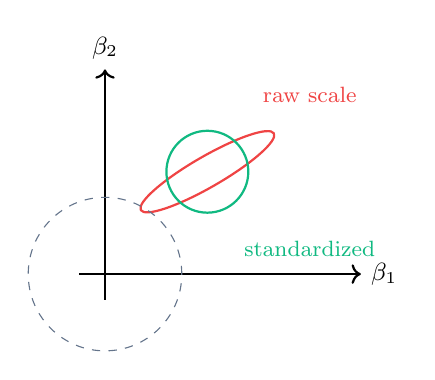
\begin{tikzpicture}[scale=0.65]
  \draw[->, thick] (-0.5,0) -- (5,0) node[right] {\small $\beta_1$};
  \draw[->, thick] (0,-0.5) -- (0,4) node[above] {\small $\beta_2$};
  % Unstandardized: elongated ellipse
  \draw[softred, thick, rotate around={30:(2,2)}] (2,2) ellipse (1.5 and 0.3);
  \node[softred, font=\footnotesize] at (4, 3.5) {raw scale};
  % Standardized: circular
  \draw[softgreen, thick] (2,2) circle (0.8);
  \node[softgreen, font=\footnotesize] at (4, 0.5) {standardized};
  % Penalty circle
  \draw[muted, dashed] (0,0) circle (1.5);
\end{tikzpicture}
\vspace{0.2em}
\footnotesize Standardized: penalty circle\\treats all directions equally
\end{columns}
\end{frame}

% ════════════ THE LASSO ════════════
\begin{frame}{The Lasso: Sparse Models}
$$\hat{\beta}^L_\lambda = \arg\min_\beta \left\{ \text{RSS} + \lambda \sum_{j=1}^p |\beta_j| \right\}$$

\begin{columns}
\column{0.5\textwidth}
\textbf{Key difference from Ridge:}

$|\beta_j|$ instead of $\beta_j^2$

$\Rightarrow$ The $\ell_1$ penalty can force coefficients to \textbf{exactly zero}!

\vspace{0.3em}
\textbf{Lasso = automatic variable selection}

At a given $\lambda$, only a \textbf{subset} of predictors survive

\vspace{0.3em}
Models are \textbf{sparse} and interpretable

\column{0.45\textwidth}
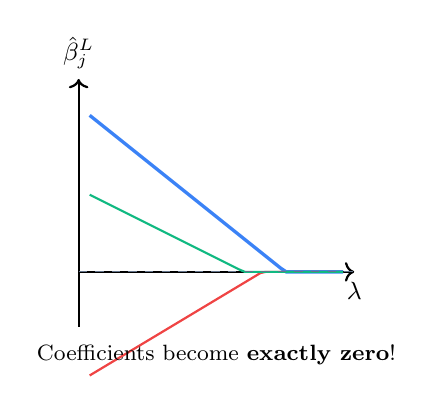
\begin{tikzpicture}[scale=0.7]
  \draw[->, thick] (0,0) -- (5,0) node[below] {\small $\lambda$};
  \draw[->, thick] (0,-1) -- (0,3.5) node[above] {\small $\hat{\beta}_j^L$};
  % Coefficients hitting zero
  \draw[accent, very thick, domain=0.2:4.8, samples=50] plot (\x, {max(3-0.8*\x, 0)});
  \draw[softred, thick, domain=0.2:4.8, samples=50] plot (\x, {min(-2+0.6*\x, 0)});
  \draw[softgreen, thick, domain=0.2:4.8, samples=50] plot (\x, {max(1.5-0.5*\x, 0)});
  \draw[muted, dashed] (0, 0) -- (5, 0);
  \node[font=\footnotesize] at (2.5, -1.5) {Coefficients become \textbf{exactly zero}!};
\end{tikzpicture}
\end{columns}
\end{frame}

\begin{frame}{Why Does Lasso Produce Zeros? The Geometry}
\begin{columns}
\column{0.48\textwidth}
\textbf{Lasso constraint:} $|\beta_1| + |\beta_2| \leq s$

Shape: \textbf{diamond}

Corners lie on axes $\Rightarrow$ solutions land at corners $\Rightarrow$ some $\beta_j = 0$

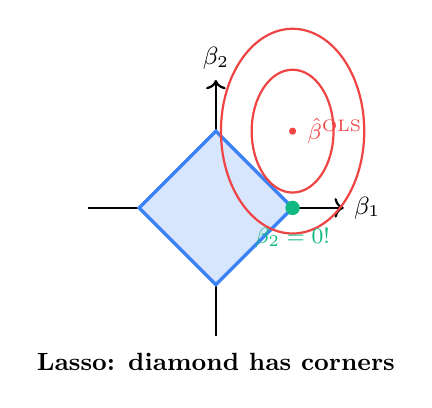
\begin{tikzpicture}[scale=0.65]
  \draw[->, thick] (-2.5,0) -- (2.5,0) node[right] {\small $\beta_1$};
  \draw[->, thick] (0,-2.5) -- (0,2.5) node[above] {\small $\beta_2$};
  % Diamond (L1)
  \fill[accent!20] (0,1.5) -- (1.5,0) -- (0,-1.5) -- (-1.5,0) -- cycle;
  \draw[accent, very thick] (0,1.5) -- (1.5,0) -- (0,-1.5) -- (-1.5,0) -- cycle;
  % Ellipses
  \draw[softred, thick] (1.5, 1.5) ellipse (0.8 and 1.2);
  \draw[softred, thick] (1.5, 1.5) ellipse (1.4 and 2.0);
  \fill[softred] (1.5, 1.5) circle (2pt);
  \node[softred, right, font=\footnotesize] at (1.6, 1.5) {$\hat{\beta}^{\text{OLS}}$};
  % Solution at corner!
  \fill[softgreen] (1.5, 0) circle (4pt);
  \node[softgreen, below, font=\footnotesize] at (1.5, -0.2) {$\beta_2 = 0$!};
  \node[font=\small\bfseries] at (0, -3) {Lasso: diamond has corners};
\end{tikzpicture}

\column{0.48\textwidth}
\textbf{Ridge constraint:} $\beta_1^2 + \beta_2^2 \leq s$

Shape: \textbf{circle}

No corners $\Rightarrow$ solutions rarely land exactly on axis

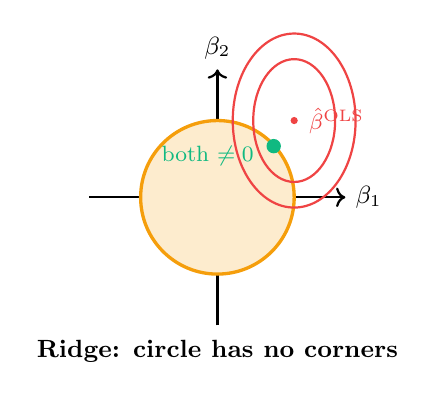
\begin{tikzpicture}[scale=0.65]
  \draw[->, thick] (-2.5,0) -- (2.5,0) node[right] {\small $\beta_1$};
  \draw[->, thick] (0,-2.5) -- (0,2.5) node[above] {\small $\beta_2$};
  % Circle (L2)
  \fill[amber!20] (0,0) circle (1.5);
  \draw[amber, very thick] (0,0) circle (1.5);
  % Ellipses
  \draw[softred, thick] (1.5, 1.5) ellipse (0.8 and 1.2);
  \draw[softred, thick] (1.5, 1.5) ellipse (1.2 and 1.7);
  \fill[softred] (1.5, 1.5) circle (2pt);
  \node[softred, right, font=\footnotesize] at (1.6, 1.5) {$\hat{\beta}^{\text{OLS}}$};
  % Solution NOT at axis
  \fill[softgreen] (1.1, 1.0) circle (4pt);
  \node[softgreen, left, font=\footnotesize] at (0.9, 0.8) {both $\neq 0$};
  \node[font=\small\bfseries] at (0, -3) {Ridge: circle has no corners};
\end{tikzpicture}
\end{columns}
\end{frame}

\begin{frame}{Ridge vs.\ Lasso: Side-by-Side}
\begin{center}
\begin{tabular}{lcc}
\toprule
Feature & Ridge & Lasso \\
\midrule
Penalty & $\lambda \sum \beta_j^2$ ($\ell_2$) & $\lambda \sum |\beta_j|$ ($\ell_1$) \\
Constraint shape & Circle & Diamond \\
Coefficients $= 0$? & \textcolor{softred}{Never} & \textcolor{softgreen}{Yes, at corners} \\
Variable selection & No & \textcolor{softgreen}{Yes} \\
Closed form & Yes & No (iterative) \\
Correlated predictors & Keeps all, shrinks evenly & Picks one, drops others \\
Best when & Many small effects & Few large effects \\
\bottomrule
\end{tabular}
\end{center}
\vspace{0.5em}
\centering
\textit{In practice, try both and use CV to decide!}
\end{frame}

\begin{frame}{The Elastic Net: Best of Both Worlds}
$$\hat{\beta}^{EN} = \arg\min_\beta \left\{ \text{RSS} + \lambda \left[\alpha \sum |\beta_j| + (1-\alpha)\sum \beta_j^2 \right]\right\}$$

\begin{columns}
\column{0.5\textwidth}
$\alpha = 1$: pure Lasso

$\alpha = 0$: pure Ridge

$\alpha \in (0,1)$: Elastic Net (compromise)

\vspace{0.3em}
\textbf{Advantages:}
\begin{itemize}
  \item Selects variables like Lasso
  \item Groups correlated variables like Ridge
  \item Often outperforms both individually
\end{itemize}

\column{0.45\textwidth}
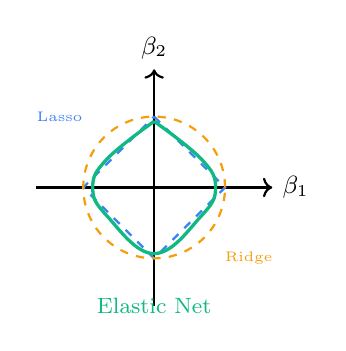
\begin{tikzpicture}[scale=0.6]
  \draw[->, thick] (-2.5,0) -- (2.5,0) node[right] {\small $\beta_1$};
  \draw[->, thick] (0,-2.5) -- (0,2.5) node[above] {\small $\beta_2$};
  % L1 (diamond)
  \draw[accent, thick, dashed] (0,1.5) -- (1.5,0) -- (0,-1.5) -- (-1.5,0) -- cycle;
  \node[accent, font=\tiny] at (-2, 1.5) {Lasso};
  % L2 (circle)
  \draw[amber, thick, dashed] (0,0) circle (1.5);
  \node[amber, font=\tiny] at (2, -1.5) {Ridge};
  % Elastic net (rounded diamond)
  \draw[softgreen, very thick, smooth, tension=0.7] plot coordinates {(0,1.4)(1.0,0.6)(1.3,0)(1.0,-0.6)(0,-1.4)(-1.0,-0.6)(-1.3,0)(-1.0,0.6)(0,1.4)};
  \node[softgreen, font=\footnotesize] at (0, -2.5) {Elastic Net};
\end{tikzpicture}
\vspace{0.2em}
\footnotesize R: \texttt{glmnet(x, y, alpha=0.5)}
\end{columns}
\end{frame}

\begin{frame}{Choosing $\lambda$: Cross-Validation}
\begin{columns}
\column{0.5\textwidth}
\textbf{Algorithm:}
\begin{enumerate}
  \item Create a grid of $\lambda$ values
  \item For each $\lambda$, compute 10-fold CV error
  \item Choose $\lambda$ with lowest CV error
  \item Or use 1-SE rule for sparser model
\end{enumerate}

\vspace{0.3em}
\texttt{cv.glmnet()} does this automatically!

\column{0.45\textwidth}
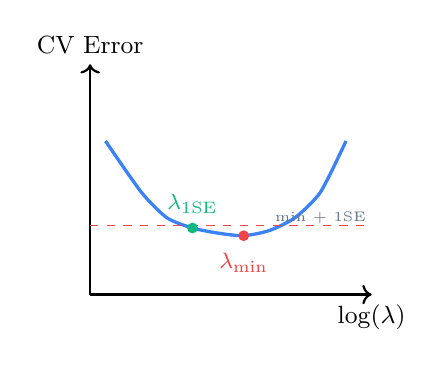
\begin{tikzpicture}[scale=0.65]
  \draw[->, thick] (0,0) -- (5.5,0) node[below] {\small $\log(\lambda)$};
  \draw[->, thick] (0,0) -- (0,4.5) node[above] {\small CV Error};
  \draw[accent, very thick, smooth, tension=0.4] plot coordinates {(0.3,3.0)(1,2.0)(1.5,1.5)(2,1.3)(2.5,1.2)(3,1.15)(3.5,1.25)(4,1.5)(4.5,2.0)(5,3.0)};
  % Min
  \fill[softred] (3, 1.15) circle (3pt);
  \node[softred, below, font=\footnotesize] at (3, 1.0) {$\lambda_{\min}$};
  % 1-SE
  \draw[softred, dashed] (0, 1.35) -- (5.5, 1.35);
  \fill[softgreen] (2, 1.3) circle (3pt);
  \node[softgreen, above, font=\footnotesize] at (2, 1.4) {$\lambda_{\text{1SE}}$};
  \node[muted, font=\tiny] at (4.5, 1.5) {min + 1SE};
\end{tikzpicture}
\vspace{0.2em}
$\lambda_{\min}$: lowest CV error

$\lambda_{\text{1SE}}$: most regularized within 1 SE
\end{columns}
\end{frame}

\begin{frame}{Worked Example: Lasso on Hitters}
\begin{columns}
\column{0.5\textwidth}
\textbf{10-fold CV on Lasso:}

$\lambda_{\min} = 9.3$ $\Rightarrow$ 15 predictors

$\lambda_{\text{1SE}} = 52.8$ $\Rightarrow$ 7 predictors

\vspace{0.3em}
\textbf{Selected predictors ($\lambda_{\text{1SE}}$):}
\begin{itemize}
  \item AtBat, Hits, Walks
  \item CRuns, CRBI, CWalks
  \item DivisionW
\end{itemize}

12 predictors \textbf{dropped}!

\column{0.45\textwidth}
\textbf{Non-zero coefficients:}
\begin{tabular}{lr}
\toprule
Predictor & $\hat{\beta}^L$ \\
\midrule
Hits & 1.39 \\
Walks & 3.23 \\
CRuns & 0.73 \\
CRBI & 0.34 \\
DivisionW & $-72.8$ \\
\bottomrule
\end{tabular}
\vspace{0.3em}
\footnotesize Sparse, interpretable model!
\end{columns}
\end{frame}

\begin{frame}{Worked Example: Ridge vs.\ Lasso on Hitters}
\begin{center}
\begin{tabular}{lccc}
\toprule
Method & CV MSE & \# Predictors & Interpretation \\
\midrule
OLS (all 19) & 141,843 & 19 & Hard \\
Best subset ($d=6$) & 130,220 & 6 & Good \\
Ridge ($\lambda_{\min}$) & 130,154 & 19 & Hard \\
\textcolor{softgreen}{Lasso ($\lambda_{\min}$)} & \textcolor{softgreen}{130,504} & \textcolor{softgreen}{15} & Medium \\
\textcolor{softgreen}{Lasso ($\lambda_{\text{1SE}}$)} & 135,012 & \textcolor{softgreen}{7} & \textcolor{softgreen}{Easy} \\
\bottomrule
\end{tabular}
\end{center}
\vspace{0.3em}
\begin{itemize}
  \item Ridge and Lasso both beat OLS substantially
  \item Ridge and Lasso give similar CV MSE
  \item Lasso is more interpretable (sparse)
  \item Best subset is competitive but doesn't scale
\end{itemize}
\end{frame}

\begin{frame}{Soft-Thresholding: The Lasso in a Special Case}
\begin{columns}
\column{0.5\textwidth}
When $\mathbf{X} = \mathbf{I}$ (orthogonal design):

\textbf{Ridge:}
$$\hat{\beta}_j^R = \frac{y_j}{1 + \lambda}$$
Proportional shrinkage

\vspace{0.3em}
\textbf{Lasso:}
$$\hat{\beta}_j^L = \text{sign}(y_j)(|y_j| - \lambda/2)_+$$
Soft thresholding: small coefficients are \textbf{zeroed out}

\column{0.45\textwidth}
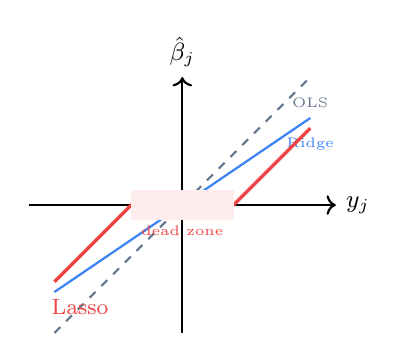
\begin{tikzpicture}[scale=0.65]
  \draw[->, thick] (-3,0) -- (3,0) node[right] {\small $y_j$};
  \draw[->, thick] (0,-2.5) -- (0,2.5) node[above] {\small $\hat{\beta}_j$};
  % OLS (45 degree line)
  \draw[muted, thick, dashed] (-2.5,-2.5) -- (2.5,2.5);
  \node[muted, font=\tiny] at (2.5, 2) {OLS};
  % Ridge
  \draw[accent, thick] (-2.5,-1.7) -- (2.5,1.7);
  \node[accent, font=\tiny] at (2.5, 1.2) {Ridge};
  % Lasso
  \draw[softred, very thick] (-2.5,-1.5) -- (-1,0) -- (1,0) -- (2.5,1.5);
  \node[softred, font=\footnotesize] at (-2, -2) {Lasso};
  % Dead zone
  \fill[softred!10] (-1,-0.3) rectangle (1,0.3);
  \node[softred, font=\tiny] at (0, -0.5) {dead zone};
\end{tikzpicture}
\vspace{0.2em}
\footnotesize Ridge: proportional shrinkage\\Lasso: threshold + shift
\end{columns}
\end{frame}

\begin{frame}{Bayesian Interpretation}
\begin{columns}
\column{0.48\textwidth}
\textbf{Ridge = Gaussian prior:}
$$\beta_j \sim N(0, \sigma^2/\lambda)$$

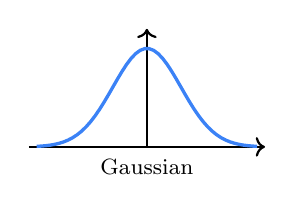
\begin{tikzpicture}[scale=0.5]
  \draw[->, thick] (-3,0) -- (3,0);
  \draw[->, thick] (0,0) -- (0,3);
  \draw[accent, very thick, domain=-2.8:2.8, samples=50] plot (\x, {2.5*exp(-\x*\x/1.5)});
  \node at (0, -0.5) {\footnotesize Gaussian};
\end{tikzpicture}

Smooth, bell-shaped prior

Most $\beta_j$ near zero, but none exactly zero

\column{0.48\textwidth}
\textbf{Lasso = Laplace prior:}
$$\beta_j \sim \text{Laplace}(0, 1/\lambda)$$

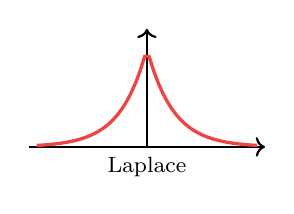
\begin{tikzpicture}[scale=0.5]
  \draw[->, thick] (-3,0) -- (3,0);
  \draw[->, thick] (0,0) -- (0,3);
  \draw[softred, very thick, domain=-2.8:2.8, samples=50] plot (\x, {2.5*exp(-1.5*abs(\x))});
  \node at (0, -0.5) {\footnotesize Laplace};
\end{tikzpicture}

Sharp peak at zero!

More probability mass at $\beta_j = 0$ $\Rightarrow$ promotes exact zeros
\end{columns}
\end{frame}

\begin{frame}{When Does Each Method Win?}
\begin{columns}
\column{0.48\textwidth}
\textbf{Lasso wins when:}
\begin{itemize}
  \item True model is sparse
  \item Only a few predictors matter
  \item Want interpretable results
  \item Feature selection is the goal
\end{itemize}

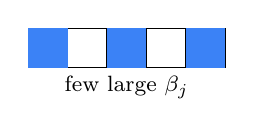
\begin{tikzpicture}[scale=0.5]
  \draw (0,0) grid (5,1);
  \fill[accent] (0,0) rectangle (1,1);
  \fill[accent] (2,0) rectangle (3,1);
  \fill[accent] (4,0) rectangle (5,1);
  \node at (2.5, -0.5) {\footnotesize few large $\beta_j$};
\end{tikzpicture}

\column{0.48\textwidth}
\textbf{Ridge wins when:}
\begin{itemize}
  \item Many predictors contribute
  \item All $\beta_j$ are roughly equal
  \item Correlated predictor groups
  \item Pure prediction is the goal
\end{itemize}

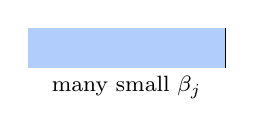
\begin{tikzpicture}[scale=0.5]
  \draw (0,0) grid (5,1);
  \fill[accent!40] (0,0) rectangle (1,1);
  \fill[accent!40] (1,0) rectangle (2,1);
  \fill[accent!40] (2,0) rectangle (3,1);
  \fill[accent!40] (3,0) rectangle (4,1);
  \fill[accent!40] (4,0) rectangle (5,1);
  \node at (2.5, -0.5) {\footnotesize many small $\beta_j$};
\end{tikzpicture}
\end{columns}

\vspace{0.5em}
\centering
\textit{In practice: try both (and elastic net), let CV decide}
\end{frame}

% ════════════ DEEP DIVES ════════════

\begin{frame}{The glmnet() Function: Anatomy}
\begin{columns}
\column{0.55\textwidth}
\footnotesize
\texttt{library(glmnet)}

\texttt{x <- model.matrix(Salary \textasciitilde{} ., data)[,-1]}

\texttt{y <- data\$Salary}

\vspace{0.2em}
\texttt{\# Ridge: alpha = 0}

\texttt{ridge <- glmnet(x, y, alpha = 0)}

\vspace{0.2em}
\texttt{\# Lasso: alpha = 1}

\texttt{lasso <- glmnet(x, y, alpha = 1)}

\vspace{0.2em}
\texttt{\# CV to choose lambda}

\texttt{cv.out <- cv.glmnet(x, y, alpha = 1)}

\texttt{best.lam <- cv.out\$lambda.min}

\texttt{coef(cv.out, s = best.lam)}
\normalsize

\column{0.4\textwidth}
\textbf{Key arguments:}

\begin{tabular}{ll}
\toprule
\texttt{alpha} & 0=Ridge, 1=Lasso \\
\texttt{lambda} & Grid of $\lambda$'s \\
\texttt{nfolds} & \# CV folds \\
\texttt{standardize} & TRUE (default) \\
\bottomrule
\end{tabular}

\vspace{0.3em}
\textbf{Key outputs:}

\texttt{lambda.min}: optimal $\lambda$

\texttt{lambda.1se}: 1-SE rule $\lambda$

\texttt{coef()}: coefficients at any $\lambda$
\end{columns}
\end{frame}

\begin{frame}{Coefficient Path Plots: Reading Them}
\begin{columns}
\column{0.5\textwidth}
\textbf{Ridge path:}
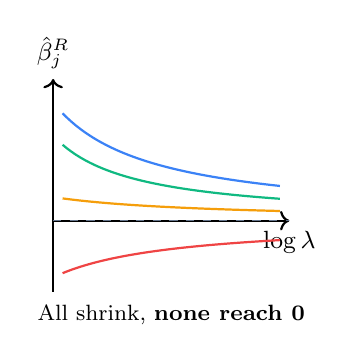
\begin{tikzpicture}[scale=0.6]
  \draw[->, thick] (0,0) -- (5,0) node[below] {\small $\log\lambda$};
  \draw[->, thick] (0,-1.5) -- (0,3) node[above] {\small $\hat{\beta}_j^R$};
  \draw[accent, thick, domain=0.2:4.8, samples=50] plot (\x, {2.5/(1+0.5*\x)});
  \draw[softred, thick, domain=0.2:4.8, samples=50] plot (\x, {-1.2/(1+0.4*\x)});
  \draw[softgreen, thick, domain=0.2:4.8, samples=50] plot (\x, {1.8/(1+0.6*\x)});
  \draw[amber, thick, domain=0.2:4.8, samples=50] plot (\x, {0.5/(1+0.3*\x)});
  \draw[muted, dashed] (0,0) -- (5,0);
  \node[font=\footnotesize] at (2.5, -2) {All shrink, \textbf{none reach 0}};
\end{tikzpicture}

\column{0.5\textwidth}
\textbf{Lasso path:}
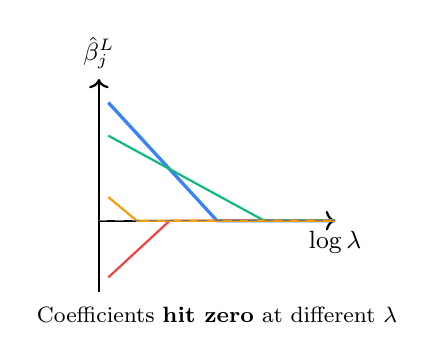
\begin{tikzpicture}[scale=0.6]
  \draw[->, thick] (0,0) -- (5,0) node[below] {\small $\log\lambda$};
  \draw[->, thick] (0,-1.5) -- (0,3) node[above] {\small $\hat{\beta}_j^L$};
  \draw[accent, very thick] (0.2, 2.5) -- (2.5, 0) -- (5, 0);
  \draw[softred, thick] (0.2, -1.2) -- (1.5, 0) -- (5, 0);
  \draw[softgreen, thick] (0.2, 1.8) -- (3.5, 0) -- (5, 0);
  \draw[amber, thick] (0.2, 0.5) -- (0.8, 0) -- (5, 0);
  \draw[muted, dashed] (0,0) -- (5,0);
  \node[font=\footnotesize] at (2.5, -2) {Coefficients \textbf{hit zero} at different $\lambda$};
\end{tikzpicture}
\end{columns}
\vspace{0.3em}
\centering
R: \texttt{plot(glmnet\_fit, xvar = "lambda")}
\end{frame}

\begin{frame}{Cross-Validation for $\lambda$: The Full Picture}
\begin{center}
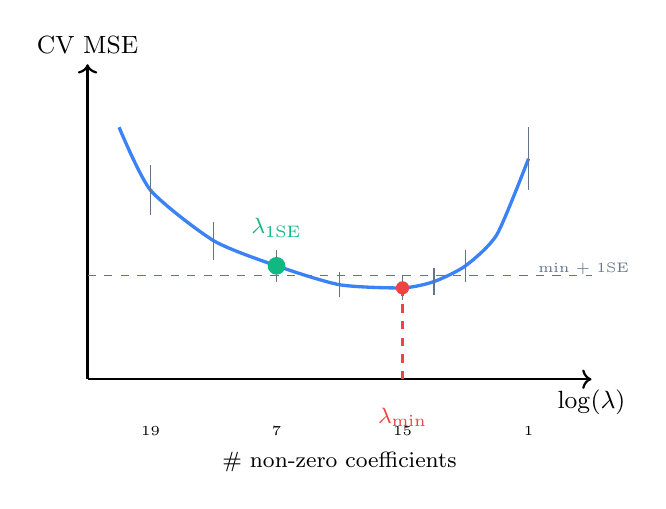
\begin{tikzpicture}[scale=0.8]
  \draw[->, thick] (0,0) -- (8,0) node[below] {\small $\log(\lambda)$};
  \draw[->, thick] (0,0) -- (0,5) node[above] {\small CV MSE};
  % CV curve with error bars
  \draw[accent, very thick, smooth, tension=0.4] plot coordinates {(0.5,4.0)(1,3.0)(2,2.2)(3,1.8)(4,1.5)(5,1.45)(5.5,1.55)(6,1.8)(6.5,2.3)(7,3.5)};
  % Error bars
  \foreach \x/\y/\se in {1/3.0/0.4, 2/2.2/0.3, 3/1.8/0.25, 4/1.5/0.2, 5/1.45/0.2, 5.5/1.55/0.22, 6/1.8/0.25, 7/3.5/0.5} {
    \draw[muted] (\x, \y-\se) -- (\x, \y+\se);
  }
  % Lambda min
  \draw[softred, thick, dashed] (5, 0) -- (5, 1.45);
  \fill[softred] (5, 1.45) circle (3pt);
  \node[softred, below, font=\footnotesize] at (5, -0.3) {$\lambda_{\min}$};
  % 1-SE line
  \draw[muted, dashed] (0, 1.65) -- (8, 1.65);
  \node[muted, right, font=\tiny] at (7, 1.75) {min + 1SE};
  % Lambda 1SE
  \fill[softgreen] (3, 1.8) circle (4pt);
  \node[softgreen, above, font=\footnotesize] at (3, 2.1) {$\lambda_{\text{1SE}}$};
  % Number of predictors
  \node[below, font=\tiny] at (1, -0.6) {19};
  \node[below, font=\tiny] at (3, -0.6) {7};
  \node[below, font=\tiny] at (5, -0.6) {15};
  \node[below, font=\tiny] at (7, -0.6) {1};
  \node[below, font=\footnotesize] at (4, -1.0) {\# non-zero coefficients};
\end{tikzpicture}
\end{center}
\end{frame}

\begin{frame}{High-Dimensional Setting: $p > n$}
\begin{columns}
\column{0.55\textwidth}
\textbf{When $p > n$:}
\begin{itemize}
  \item OLS has \textbf{no unique solution}
  \item $\mathbf{X}^T\mathbf{X}$ is singular
  \item Training RSS $= 0$ trivially (overfitting)
  \item $R^2 = 1$ meaningless!
\end{itemize}
\vspace{0.3em}
\textbf{Ridge and Lasso still work:}
\begin{itemize}
  \item $(\mathbf{X}^T\mathbf{X} + \lambda\mathbf{I})$ is always invertible (Ridge)
  \item Lasso selects at most $n$ predictors
  \item Regularization is \textbf{essential} here
\end{itemize}
\column{0.4\textwidth}
\textbf{Example:}

Genomics: $n = 100$ patients, $p = 10{,}000$ genes

\vspace{0.3em}
\begin{tabular}{lc}
\toprule
Method & Possible? \\
\midrule
OLS & \textcolor{softred}{No} \\
Best subset & \textcolor{softred}{No} \\
Forward step. & \textcolor{softgreen}{Yes} \\
Ridge & \textcolor{softgreen}{Yes} \\
Lasso & \textcolor{softgreen}{Yes} \\
\bottomrule
\end{tabular}
\end{columns}
\end{frame}

\begin{frame}{Handling Correlated Predictors}
\begin{columns}
\column{0.5\textwidth}
\textbf{Lasso with correlated predictors:}

If $X_1 \approx X_2$:

Lasso picks one and drops the other

Which one? \textbf{Essentially random!}

\vspace{0.5em}
\textbf{Ridge with correlated predictors:}

Keeps both, shrinks evenly

More stable, but less sparse

\vspace{0.5em}
\textbf{Elastic Net:}

Groups correlated variables together

Best of both worlds

\column{0.45\textwidth}
\textbf{Hitters: CRuns and CHits}

$r = 0.96$ (highly correlated!)

\vspace{0.3em}
\begin{tabular}{lcc}
\toprule
& CRuns & CHits \\
\midrule
OLS & 1.61 & $-0.13$ \\
Ridge & 0.82 & 0.71 \\
Lasso & \textcolor{softgreen}{0.73} & \textcolor{softred}{0} \\
\bottomrule
\end{tabular}

\vspace{0.3em}
OLS: unstable (opposite signs!)

Ridge: stable, similar coefficients

Lasso: picks CRuns, drops CHits
\end{columns}
\end{frame}

\begin{frame}{PCR: Principal Components Regression (Preview)}
\begin{columns}
\column{0.55\textwidth}
\textbf{Idea:}
\begin{enumerate}
  \item Compute PCA on $\mathbf{X}$ (Week 10)
  \item Keep first $M < p$ components
  \item Regress $Y$ on these $M$ components
\end{enumerate}

\vspace{0.3em}
\textbf{Advantage:}

Reduces $p$ predictors to $M$ uncorrelated components

\vspace{0.3em}
\textbf{Disadvantage:}

Components are linear combinations of all $X_j$ $\Rightarrow$ no variable selection

Choosing $M$ via CV

\column{0.4\textwidth}
\textbf{Hitters: PCR results}

\begin{tabular}{cc}
\toprule
$M$ & CV MSE \\
\midrule
1 & 188,000 \\
4 & 145,000 \\
\textcolor{softgreen}{7} & \textcolor{softgreen}{131,000} \\
19 (OLS) & 141,000 \\
\bottomrule
\end{tabular}

\vspace{0.3em}
$M = 7$ components capture most of the predictive power

\vspace{0.3em}
\footnotesize R: \texttt{pls::pcr(y \textasciitilde{} ., ncomp=7)}
\end{columns}
\end{frame}

\begin{frame}{Regularization: The Big Picture}
\begin{center}
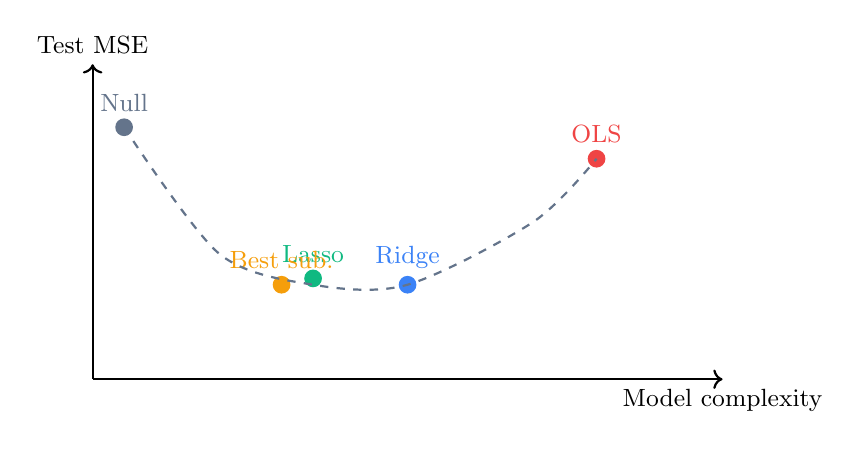
\begin{tikzpicture}[scale=0.8]
  \draw[->, thick] (0,0) -- (10,0) node[below] {\small Model complexity};
  \draw[->, thick] (0,0) -- (0,5) node[above] {\small Test MSE};
  % OLS
  \fill[softred] (8, 3.5) circle (4pt);
  \node[softred, above] at (8, 3.6) {\small OLS};
  % Ridge
  \fill[accent] (5, 1.5) circle (4pt);
  \node[accent, above] at (5, 1.6) {\small Ridge};
  % Lasso
  \fill[softgreen] (3.5, 1.6) circle (4pt);
  \node[softgreen, above] at (3.5, 1.7) {\small Lasso};
  % Best subset
  \fill[amber] (3, 1.5) circle (4pt);
  \node[amber, above] at (3, 1.6) {\small Best sub.};
  % Null model
  \fill[muted] (0.5, 4) circle (4pt);
  \node[muted, above] at (0.5, 4.1) {\small Null};
  % Curve
  \draw[muted, thick, dashed, smooth, tension=0.5] plot coordinates {(0.5,4)(2,2)(3.5,1.5)(5,1.5)(7,2.5)(8,3.5)};
\end{tikzpicture}
\end{center}
\vspace{0.3em}
Regularization finds the \textbf{sweet spot} between the null model (too simple) and full OLS (too complex)
\end{frame}

\begin{frame}{Think: What Does $\lambda = 0$ vs.\ $\lambda = \infty$ Give You?}
\begin{columns}
\column{0.48\textwidth}
\textbf{$\lambda = 0$:} No penalty

$\hat{\beta}^R = \hat{\beta}^{\text{OLS}}$

Full model, no shrinkage

Maximum variance, minimum bias

\vspace{0.5em}
\textbf{$\lambda = \infty$:} Maximum penalty

$\hat{\beta}^R \to 0$ (all coefficients)

Null model: $\hat{Y} = \bar{Y}$

Minimum variance, maximum bias

\column{0.48\textwidth}
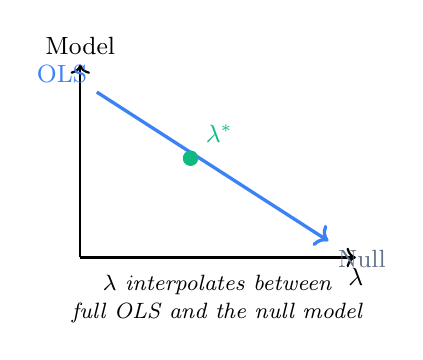
\begin{tikzpicture}[scale=0.7]
  \draw[->, thick] (0,0) -- (5,0) node[below] {\small $\lambda$};
  \draw[->, thick] (0,0) -- (0,3.5) node[above] {\small Model};
  % Arrow from OLS to null
  \draw[very thick, accent, ->] (0.3, 3) -- (4.5, 0.3);
  \node[accent, above left] at (0.3, 3) {\small OLS};
  \node[muted, below right] at (4.5, 0.3) {\small Null};
  % Star
  \fill[softgreen] (2, 1.8) circle (4pt);
  \node[softgreen, above right] at (2.1, 1.9) {\small $\lambda^*$};
  \node[font=\footnotesize] at (2.5, -0.5) {\textit{$\lambda$ interpolates between}};
  \node[font=\footnotesize] at (2.5, -1) {\textit{full OLS and the null model}};
\end{tikzpicture}
\end{columns}
\end{frame}

\begin{frame}{Worked Example: Ridge on Hitters (Numerical)}
\textbf{At $\lambda = 0$ (OLS):}

$\hat{\beta}_{\text{AtBat}} = -1.98$, $\hat{\beta}_{\text{Hits}} = 7.50$, $\hat{\beta}_{\text{Walks}} = 6.06$

\vspace{0.3em}
\textbf{At $\lambda = 100$:}

$\hat{\beta}_{\text{AtBat}} = -0.71$, $\hat{\beta}_{\text{Hits}} = 2.73$, $\hat{\beta}_{\text{Walks}} = 2.69$

\vspace{0.3em}
\textbf{At $\lambda = 10{,}000$:}

$\hat{\beta}_{\text{AtBat}} = -0.005$, $\hat{\beta}_{\text{Hits}} = 0.011$, $\hat{\beta}_{\text{Walks}} = 0.012$

\vspace{0.5em}
\centering
\begin{tabular}{lccc}
\toprule
$\lambda$ & $\|\hat{\beta}\|_2$ & \# nonzero & CV MSE \\
\midrule
0 (OLS) & 228 & 19 & 141,843 \\
\textcolor{softgreen}{100} & \textcolor{softgreen}{89} & \textcolor{softgreen}{19} & \textcolor{softgreen}{130,154} \\
10,000 & 2.3 & 19 & 178,500 \\
\bottomrule
\end{tabular}
\end{frame}

\begin{frame}{Ridge: Worked Numerical Example (Mini Data)}
\begin{columns}
\column{0.48\textwidth}
\textbf{Tiny data:} $n = 4$, $p = 2$

\begin{tabular}{ccc}
\toprule
$x_1$ & $x_2$ & $y$ \\
\midrule
1 & 2 & 5 \\
2 & 1 & 4 \\
3 & 3 & 8 \\
4 & 2 & 7 \\
\bottomrule
\end{tabular}

(Already centered \& standardized)

\column{0.48\textwidth}
\textbf{OLS:} $\hat{\beta} = (1.4, 0.8)$

\textbf{Ridge at $\lambda = 1$:}

$\hat{\beta}^R = (\mathbf{X}^T\mathbf{X} + \mathbf{I})^{-1}\mathbf{X}^T\mathbf{y}$

$= (1.15, 0.65)$ \quad (shrunken!)

\textbf{Ridge at $\lambda = 10$:}

$= (0.52, 0.30)$ \quad (more shrinkage)

\vspace{0.3em}
\textit{Both coefficients approach zero\\as $\lambda$ grows, but neither reaches 0}
\end{columns}
\end{frame}


\begin{frame}{Lasso: Worked Numerical Example}
\begin{columns}
\column{0.48\textwidth}
\textbf{Same data, Lasso:}

\textbf{OLS:} $\hat{\beta} = (1.4, 0.8)$

\textbf{Lasso at $\lambda = 0.5$:}

$\hat{\beta}^L = (1.15, 0.55)$

\textbf{Lasso at $\lambda = 1.5$:}

$\hat{\beta}^L = (0.65, \textcolor{softred}{0})$ \quad \textcolor{softred}{$x_2$ dropped!}

\textbf{Lasso at $\lambda = 3$:}

$\hat{\beta}^L = (\textcolor{softred}{0}, \textcolor{softred}{0})$ \quad Null model

\column{0.48\textwidth}
\textbf{Timeline:}

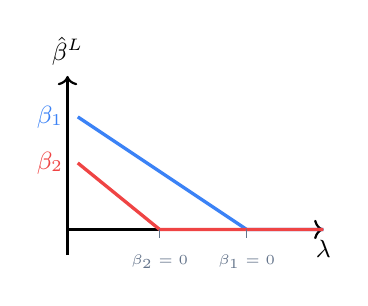
\begin{tikzpicture}[scale=0.65]
  \draw[->, thick] (0,0) -- (5,0) node[below] {\small $\lambda$};
  \draw[->, thick] (0,-0.5) -- (0,3) node[above] {\small $\hat{\beta}^L$};
  % beta_1
  \draw[accent, very thick] (0.2, 2.2) -- (3.5, 0) -- (5, 0);
  \node[accent, left] at (0.1, 2.2) {\small $\beta_1$};
  % beta_2
  \draw[softred, very thick] (0.2, 1.3) -- (1.8, 0) -- (5, 0);
  \node[softred, left] at (0.1, 1.3) {\small $\beta_2$};
  % Annotations
  \draw[muted, dashed] (1.8, 0) -- (1.8, -0.3);
  \node[muted, below, font=\tiny] at (1.8, -0.3) {$\beta_2=0$};
  \draw[muted, dashed] (3.5, 0) -- (3.5, -0.3);
  \node[muted, below, font=\tiny] at (3.5, -0.3) {$\beta_1=0$};
\end{tikzpicture}

$x_2$ drops first (smaller OLS coefficient)
\end{columns}
\end{frame}


\begin{frame}{Interpreting the CV Plot from \texttt{cv.glmnet}}
\begin{center}
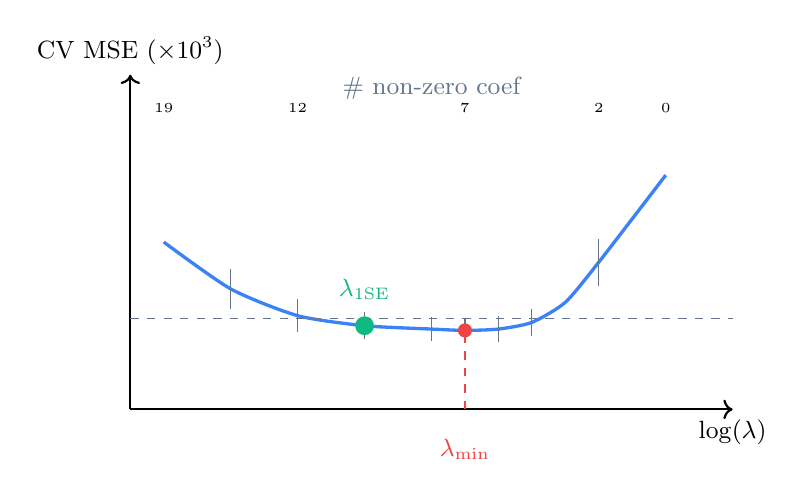
\begin{tikzpicture}[scale=0.85]
  \draw[->, thick] (0,0) -- (9,0) node[below] {\small $\log(\lambda)$};
  \draw[->, thick] (0,0) -- (0,5) node[above] {\small CV MSE ($\times 10^3$)};
  % CV curve
  \draw[accent, very thick, smooth, tension=0.4] plot coordinates {(0.5,2.5)(1.5,1.8)(2.5,1.4)(3.5,1.25)(4.5,1.2)(5,1.18)(5.5,1.2)(6,1.3)(6.5,1.6)(7,2.2)(8,3.5)};
  % Error bars
  \foreach \x/\y/\se in {1.5/1.8/0.3, 2.5/1.4/0.25, 3.5/1.25/0.2, 4.5/1.2/0.18, 5/1.18/0.18, 5.5/1.2/0.19, 6/1.3/0.2, 7/2.2/0.35} {
    \draw[muted] (\x, \y-\se) -- (\x, \y+\se);
  }
  % Lambda min
  \draw[softred, thick, dashed] (5, 0) -- (5, 1.18);
  \fill[softred] (5, 1.18) circle (3pt);
  \node[softred, below, font=\small] at (5, -0.3) {$\lambda_{\min}$};
  % 1-SE rule
  \draw[muted, dashed] (0, 1.36) -- (9, 1.36);
  \fill[softgreen] (3.5, 1.25) circle (4pt);
  \node[softgreen, above, font=\small] at (3.5, 1.5) {$\lambda_{\text{1SE}}$};
  % Top: number of variables
  \node[font=\tiny] at (0.5, 4.5) {19};
  \node[font=\tiny] at (2.5, 4.5) {12};
  \node[font=\tiny] at (5, 4.5) {7};
  \node[font=\tiny] at (7, 4.5) {2};
  \node[font=\tiny] at (8, 4.5) {0};
  \node[font=\small, muted] at (4.5, 4.8) {\# non-zero coef};
\end{tikzpicture}
\end{center}
\begin{itemize}
  \item Top axis: \# predictors surviving at each $\lambda$
  \item Vertical bars: $\pm 1$ standard error of the CV estimate
  \item Left dashed line: $\lambda_{\min}$ (minimum CV error)
  \item Right dashed line: $\lambda_{\text{1SE}}$ (most regularized within 1 SE)
\end{itemize}
\end{frame}


\begin{frame}{The $\ell_1$ vs.\ $\ell_2$ Norm: Visual Intuition}
\begin{columns}
\column{0.48\textwidth}
\textbf{$\ell_1$ norm (Lasso):}
$$\|\beta\|_1 = |\beta_1| + |\beta_2|$$
``Taxi-cab distance''

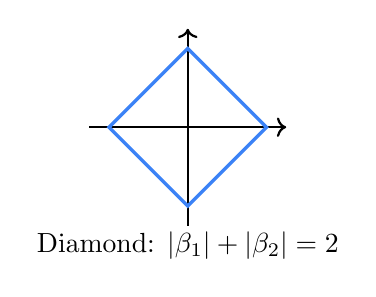
\begin{tikzpicture}[scale=0.5]
  \draw[->, thick] (-2.5,0) -- (2.5,0);
  \draw[->, thick] (0,-2.5) -- (0,2.5);
  \draw[accent, very thick] (0,2) -- (2,0) -- (0,-2) -- (-2,0) -- cycle;
  \node at (0, -3) {Diamond: $|\beta_1|+|\beta_2| = 2$};
\end{tikzpicture}

\column{0.48\textwidth}
\textbf{$\ell_2$ norm (Ridge):}
$$\|\beta\|_2 = \sqrt{\beta_1^2 + \beta_2^2}$$
``Euclidean distance''

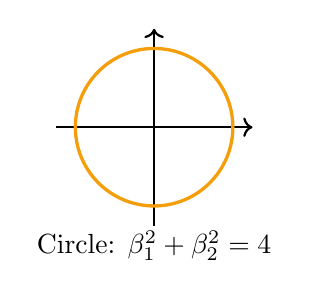
\begin{tikzpicture}[scale=0.5]
  \draw[->, thick] (-2.5,0) -- (2.5,0);
  \draw[->, thick] (0,-2.5) -- (0,2.5);
  \draw[amber, very thick] (0,0) circle (2);
  \node at (0, -3) {Circle: $\beta_1^2+\beta_2^2 = 4$};
\end{tikzpicture}
\end{columns}

\centering
\vspace{0.3em}
The diamond has \textbf{sharp corners} on the axes --- that's why Lasso produces zeros!
\end{frame}


\begin{frame}{The Constraint Formulation: A Different View}
\begin{columns}
\column{0.5\textwidth}
\textbf{Equivalent formulations:}

\textbf{Ridge:}
$$\min_\beta \text{RSS} \quad \text{subject to} \quad \sum \beta_j^2 \leq s$$

\textbf{Lasso:}
$$\min_\beta \text{RSS} \quad \text{subject to} \quad \sum |\beta_j| \leq s$$

For every $\lambda$, there exists an $s$ that gives the same solution

\column{0.45\textwidth}
\textbf{Intuition:}

``Minimize RSS while keeping coefficients small''

\vspace{0.3em}
Small $s$ $\Rightarrow$ tight constraint $\Rightarrow$ lots of shrinkage (large $\lambda$)

Large $s$ $\Rightarrow$ loose constraint $\Rightarrow$ little shrinkage ($\lambda \approx 0$)

\vspace{0.3em}
If $s$ is large enough: constraint is not binding $\Rightarrow$ OLS solution
\end{columns}
\end{frame}


\begin{frame}{Best Subset vs.\ Lasso: Computational Comparison}
\begin{center}
\begin{tabular}{lcccc}
\toprule
 & Best Subset & Forward & Lasso & Ridge \\
\midrule
Computation & $O(2^p)$ & $O(p^2)$ & $O(p \cdot n)$ & $O(p \cdot n)$ \\
$p = 10$ & 1,024 & 55 & fast & fast \\
$p = 20$ & 1M & 210 & fast & fast \\
$p = 100$ & impossible & 5,050 & fast & fast \\
$p = 10{,}000$ & impossible & 50M & fast & fast \\
$p > n$? & No & Yes & Yes & Yes \\
Selects vars? & Yes & Yes & Yes & No \\
\bottomrule
\end{tabular}
\end{center}

\vspace{0.3em}
\textbf{Key insight:} \texttt{glmnet()} fits the \textbf{entire regularization path} (all $\lambda$'s) in about the same time as a single OLS fit!
\end{frame}


\begin{frame}{Standardization: Before and After}
\begin{columns}
\column{0.5\textwidth}
\textbf{Before standardization:}

Income: range \$10k--\$100k

Age: range 20--70

$\hat{\beta}_{\text{income}} = 0.0001$ (tiny!)

$\hat{\beta}_{\text{age}} = 50$ (huge!)

Penalty: $0.0001^2 + 50^2 = 2500$

$\Rightarrow$ Age is penalized \textbf{much more}!

\column{0.45\textwidth}
\textbf{After standardization:}

$\tilde{X}_{\text{income}}$: mean 0, SD 1

$\tilde{X}_{\text{age}}$: mean 0, SD 1

$\hat{\beta}_{\text{income}} = 0.35$

$\hat{\beta}_{\text{age}} = 0.42$

Penalty: $0.35^2 + 0.42^2 = 0.30$

$\Rightarrow$ Both treated \textbf{equally}!
\end{columns}

\vspace{0.5em}
\centering
\texttt{glmnet()} standardizes by default (\texttt{standardize = TRUE})

Coefficients are returned on the \textbf{original} scale
\end{frame}


\begin{frame}{Forward Selection: Step-by-Step on Hitters}
\begin{columns}
\column{0.55\textwidth}
\textbf{Step 0:} Null model ($\bar{y}$)

\textbf{Step 1:} Try all 19 single-predictor models

Best: CRBI ($R^2 = 0.321$)

\vspace{0.2em}
\textbf{Step 2:} Fix CRBI, try adding each of 18 remaining

Best: CRBI + Hits ($R^2 = 0.426$)

\vspace{0.2em}
\textbf{Step 3:} Best addition: PutOuts ($R^2 = 0.458$)

$\vdots$

\textbf{Step 6:} BIC minimum reached (6 predictors)

\column{0.4\textwidth}
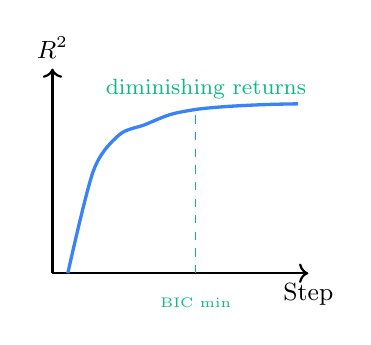
\begin{tikzpicture}[scale=0.65]
  \draw[->, thick] (0,0) -- (5,0) node[below] {\small Step};
  \draw[->, thick] (0,0) -- (0,4) node[above] {\small $R^2$};
  \draw[accent, very thick, smooth, tension=0.5] plot coordinates {(0.3,0)(0.8,2.0)(1.3,2.7)(1.8,2.9)(2.3,3.1)(2.8,3.2)(3.3,3.25)(3.8,3.28)(4.3,3.3)(4.8,3.31)};
  \node[softgreen, font=\footnotesize] at (3, 3.6) {diminishing returns};
  \draw[softgreen, dashed] (2.8, 0) -- (2.8, 3.2);
  \node[softgreen, below, font=\tiny] at (2.8, -0.3) {BIC min};
\end{tikzpicture}

\vspace{0.3em}
\footnotesize R: \texttt{regsubsets(Salary \textasciitilde{} .,}

\texttt{\quad data, method="forward")}
\end{columns}
\end{frame}


\begin{frame}{$C_p$, BIC, Adj.~$R^2$: Hitters Results}
\begin{center}
\begin{tabular}{ccccc}
\toprule
\# Predictors & RSS & $C_p$ & BIC & Adj.~$R^2$ \\
\midrule
1 & 36,180 & 104 & $-90$ & 0.321 \\
2 & 33,420 & 56 & $-128$ & 0.411 \\
4 & 30,750 & 18 & $-142$ & 0.444 \\
\textcolor{softgreen}{6} & 29,850 & 8 & \textcolor{softgreen}{$-148$} & 0.452 \\
8 & 29,380 & 7 & $-144$ & 0.457 \\
\textcolor{accent}{10} & 29,050 & \textcolor{accent}{4} & $-140$ & \textcolor{accent}{0.460} \\
19 & 28,510 & 20 & $-110$ & 0.454 \\
\bottomrule
\end{tabular}
\end{center}
\begin{itemize}
  \item BIC picks 6 predictors (harshest penalty)
  \item $C_p$ picks 10 predictors
  \item Adj.~$R^2$ picks 11 predictors (mildest penalty)
  \item All agree: OLS with all 19 is too many
\end{itemize}
\end{frame}


\begin{frame}{The $\lambda$ Path: What \texttt{glmnet} Actually Computes}
\begin{columns}
\column{0.55\textwidth}
\texttt{glmnet()} doesn't fit a single model --- it fits models for a \textbf{grid of 100 $\lambda$ values} simultaneously!

\vspace{0.3em}
\textbf{The trick: Warm starts}

Start at $\lambda_{\max}$ (all $\hat{\beta} = 0$)

Decrease $\lambda$ gradually

Use previous solution as starting point

$\Rightarrow$ Each step is very fast!

\vspace{0.3em}
Total cost $\approx$ same as one OLS fit

\column{0.4\textwidth}
\textbf{$\lambda$ grid:}

$\lambda_{\max}$: smallest $\lambda$ where all $\hat{\beta} = 0$

$$\lambda_{\max} = \frac{1}{n}\max_j |X_j^T y|$$

$\lambda_{\min} = \epsilon \cdot \lambda_{\max}$

(default $\epsilon = 0.0001$)

\vspace{0.3em}
100 values on log scale between $\lambda_{\max}$ and $\lambda_{\min}$
\end{columns}
\end{frame}


\begin{frame}{Degrees of Freedom: Ridge vs.\ Lasso}
\begin{columns}
\column{0.5\textwidth}
\textbf{OLS:} df $= p$ (always)

\textbf{Ridge:}
$$\text{df}(\lambda) = \sum_{j=1}^p \frac{d_j^2}{d_j^2 + \lambda}$$

where $d_j$ are singular values of $\mathbf{X}$

$\lambda = 0$: df $= p$ (OLS)

$\lambda \to \infty$: df $\to 0$ (null model)

Continuous, between 0 and $p$

\column{0.45\textwidth}
\textbf{Lasso:}

df $\approx$ number of non-zero coefficients

A discrete, interpretable quantity

\vspace{0.5em}
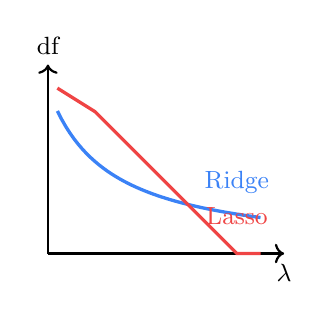
\begin{tikzpicture}[scale=0.6]
  \draw[->, thick] (0,0) -- (5,0) node[below] {\small $\lambda$};
  \draw[->, thick] (0,0) -- (0,4) node[above] {\small df};
  \draw[accent, very thick, domain=0.2:4.5, samples=50] plot (\x, {3.5/(1+0.8*\x)});
  \node[accent] at (4, 1.5) {\small Ridge};
  \draw[softred, very thick] (0.2, 3.5) -- (1, 3) -- (1.5, 2.5) -- (2, 2) -- (2.5, 1.5) -- (3, 1) -- (3.5, 0.5) -- (4, 0) -- (4.5, 0);
  \node[softred] at (4, 0.8) {\small Lasso};
\end{tikzpicture}
\end{columns}
\end{frame}


\begin{frame}{Elastic Net: Grouping Effect}
\begin{columns}
\column{0.55\textwidth}
\textbf{The Lasso problem:}

With correlated predictors $X_1 \approx X_2$:

Lasso picks one, drops the other (random)

$\Rightarrow$ Unstable selection

\vspace{0.5em}
\textbf{Elastic Net solves this:}

The $\ell_2$ component encourages correlated predictors to have similar coefficients

$\Rightarrow$ They are selected/dropped \textbf{together}

$\Rightarrow$ More stable variable selection

\column{0.4\textwidth}
\textbf{Example:}

$X_1$ and $X_2$ have $r = 0.95$

\begin{tabular}{lcc}
\toprule
 & $\hat{\beta}_1$ & $\hat{\beta}_2$ \\
\midrule
Lasso & 1.2 & \textcolor{softred}{0} \\
EN ($\alpha$=0.5) & 0.7 & 0.6 \\
Ridge & 0.5 & 0.5 \\
\bottomrule
\end{tabular}

\vspace{0.3em}
Elastic Net: both survive!

Coefficients are similar (grouped)
\end{columns}
\end{frame}


\begin{frame}{Regularization as a Bias-Variance Slider}
\begin{center}
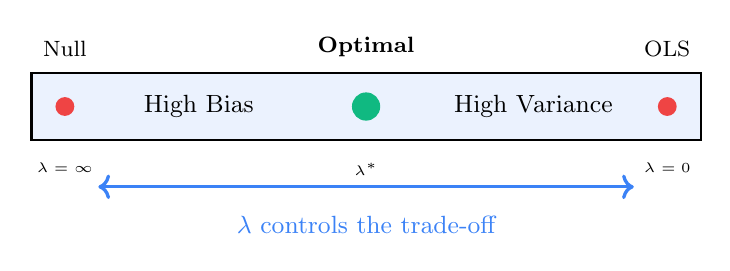
\begin{tikzpicture}[scale=0.85]
  % Slider
  \fill[accent!10] (0, 2) rectangle (10, 3);
  \draw[thick] (0, 2) rectangle (10, 3);
  % Markers
  \fill[softred] (0.5, 2.5) circle (4pt);
  \node[above, font=\footnotesize] at (0.5, 3.1) {Null};
  \node[below, font=\tiny] at (0.5, 1.8) {$\lambda=\infty$};
  \fill[softgreen] (5, 2.5) circle (6pt);
  \node[above, font=\footnotesize\bfseries] at (5, 3.1) {Optimal};
  \node[below, font=\tiny] at (5, 1.8) {$\lambda^*$};
  \fill[softred] (9.5, 2.5) circle (4pt);
  \node[above, font=\footnotesize] at (9.5, 3.1) {OLS};
  \node[below, font=\tiny] at (9.5, 1.8) {$\lambda=0$};
  % Labels
  \node[font=\small] at (2.5, 2.5) {High Bias};
  \node[font=\small] at (2.5, 2) {};
  \node[font=\small] at (7.5, 2.5) {High Variance};
  % Arrow
  \draw[<->, very thick, accent] (1, 1.3) -- (9, 1.3);
  \node[accent, below, font=\small] at (5, 1.0) {$\lambda$ controls the trade-off};
\end{tikzpicture}
\end{center}

\vspace{0.3em}
\textbf{CV finds the sweet spot} where total prediction error (bias$^2$ + variance) is minimized
\end{frame}


\begin{frame}{Common Mistakes with Regularization}
\begin{enumerate}
  \item \textbf{Forgetting to standardize}
  \begin{itemize}
    \item[$\circ$] Penalty is not scale-invariant! \texttt{glmnet} does it by default
  \end{itemize}
  \vspace{0.2em}
  \item \textbf{Including the intercept in the penalty}
  \begin{itemize}
    \item[$\circ$] The intercept $\beta_0$ should \textbf{not} be penalized (it's just the mean)
    \item[$\circ$] \texttt{glmnet} handles this correctly
  \end{itemize}
  \vspace{0.2em}
  \item \textbf{Using training MSE to select $\lambda$}
  \begin{itemize}
    \item[$\circ$] Always use \textbf{cross-validation}!
  \end{itemize}
  \vspace{0.2em}
  \item \textbf{Reporting $R^2$ from regularized fit}
  \begin{itemize}
    \item[$\circ$] $R^2$ doesn't penalize for $\lambda$ --- use CV MSE instead
  \end{itemize}
  \vspace{0.2em}
  \item \textbf{Confusing $\alpha$ and $\lambda$ in \texttt{glmnet}}
  \begin{itemize}
    \item[$\circ$] $\alpha$ = Ridge(0) vs Lasso(1). $\lambda$ = amount of regularization
  \end{itemize}
\end{enumerate}
\end{frame}


\begin{frame}{Connecting to Week 3: CV is Essential Here}
\begin{columns}
\column{0.55\textwidth}
\textbf{Week 3 gave us the tools:}

10-fold CV estimates test error for any $\lambda$

\textbf{Week 4 uses those tools to:}
\begin{itemize}
  \item Choose $\lambda$ for Ridge/Lasso
  \item Choose $\alpha$ for Elastic Net
  \item Choose \# predictors for subset selection
  \item Choose $M$ for PCR
\end{itemize}

\vspace{0.3em}
\textbf{Without CV, regularization is useless!}

(No way to choose $\lambda$)

\column{0.4\textwidth}
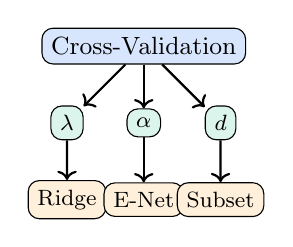
\begin{tikzpicture}[scale=0.65]
  \node[draw, fill=accent!20, rounded corners, font=\small] (cv) at (0, 3) {Cross-Validation};
  \node[draw, fill=softgreen!15, rounded corners, font=\footnotesize] (lam) at (-1.5, 1.5) {$\lambda$};
  \node[draw, fill=softgreen!15, rounded corners, font=\footnotesize] (alp) at (0, 1.5) {$\alpha$};
  \node[draw, fill=softgreen!15, rounded corners, font=\footnotesize] (d) at (1.5, 1.5) {$d$};
  \node[draw, fill=amber!15, rounded corners, font=\footnotesize] (rid) at (-1.5, 0) {Ridge};
  \node[draw, fill=amber!15, rounded corners, font=\footnotesize] (en) at (0, 0) {E-Net};
  \node[draw, fill=amber!15, rounded corners, font=\footnotesize] (sub) at (1.5, 0) {Subset};
  \draw[->, thick] (cv) -- (lam);
  \draw[->, thick] (cv) -- (alp);
  \draw[->, thick] (cv) -- (d);
  \draw[->, thick] (lam) -- (rid);
  \draw[->, thick] (alp) -- (en);
  \draw[->, thick] (d) -- (sub);
\end{tikzpicture}

\vspace{0.3em}
\textit{CV is the universal tuning tool}
\end{columns}
\end{frame}


\begin{frame}{Model Matrix: Converting Factors to Numerics}
\begin{columns}
\column{0.55\textwidth}
\texttt{glmnet()} requires a \textbf{numeric matrix}, not a data frame with factors

\vspace{0.3em}
\textbf{\texttt{model.matrix()} converts:}

\begin{itemize}
  \item Factors $\to$ dummy variables
  \item Removes intercept column (the $-1$)
  \item Keeps numeric columns as-is
\end{itemize}

\vspace{0.3em}
\footnotesize
\texttt{x <- model.matrix(Salary \textasciitilde{} .,}

\texttt{\quad\quad data = Hitters)[, -1]}

\texttt{y <- Hitters\$Salary}
\normalsize

\column{0.4\textwidth}
\textbf{Example:}

League: A, N $\Rightarrow$ LeagueN (0/1)

Division: E, W $\Rightarrow$ DivisionW (0/1)

NewLeague: A, N $\Rightarrow$ NewLeagueN (0/1)

\vspace{0.3em}
19 predictors become 19 columns

(3 factors $\to$ 3 dummies + 16 numeric)
\end{columns}
\end{frame}


\begin{frame}{Prediction with Regularized Models}
\begin{columns}
\column{0.55\textwidth}
\textbf{After choosing $\lambda^*$:}

\footnotesize
\texttt{best.lam <- cv.out\$lambda.min}

\texttt{pred <- predict(lasso.mod,}

\texttt{\quad s = best.lam, newx = x.test)}

\texttt{mse <- mean((y.test - pred)\^{}2)}
\normalsize

\vspace{0.3em}
\textbf{Extract final coefficients:}

\footnotesize
\texttt{coef(cv.out, s = "lambda.min")}

\texttt{coef(cv.out, s = "lambda.1se")}
\normalsize

\column{0.4\textwidth}
\textbf{Typical results:}

\begin{tabular}{lr}
\toprule
Predictor & $\hat{\beta}^L$ \\
\midrule
Hits & 1.39 \\
Walks & 3.23 \\
CRuns & 0.73 \\
CRBI & 0.34 \\
DivisionW & $-72.8$ \\
\textcolor{muted}{(12 others)} & \textcolor{muted}{0} \\
\bottomrule
\end{tabular}

\vspace{0.2em}
\footnotesize Sparse: only 7 of 19 survive!
\end{columns}
\end{frame}


\begin{frame}{Ridge vs.\ Lasso vs.\ OLS: The Final Showdown}
\begin{center}
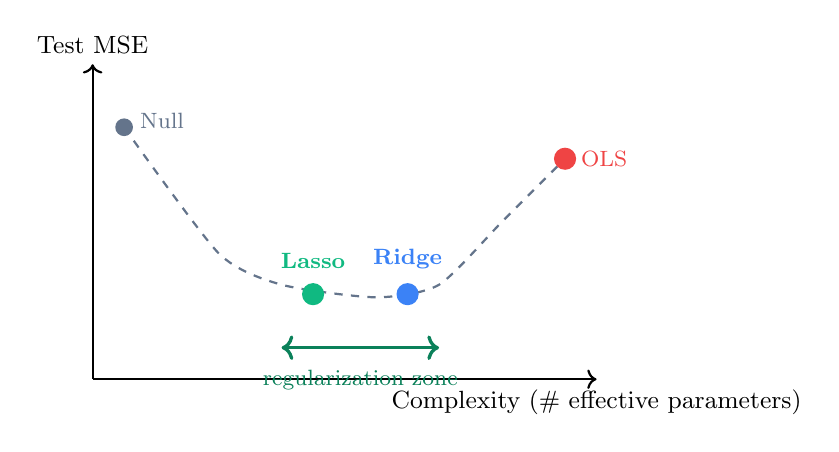
\begin{tikzpicture}[scale=0.8]
  \draw[->, thick] (0,0) -- (8,0) node[below] {\small Complexity (\# effective parameters)};
  \draw[->, thick] (0,0) -- (0,5) node[above] {\small Test MSE};
  % U-curve
  \draw[muted, thick, dashed, smooth, tension=0.4] plot coordinates {(0.5,4)(2,2)(3,1.5)(4.5,1.3)(5.5,1.5)(6.5,2.5)(7.5,3.5)};
  % Methods
  \fill[muted] (0.5, 4) circle (4pt);
  \node[muted, right, font=\footnotesize] at (0.6, 4.1) {Null};
  \fill[softgreen] (3.5, 1.35) circle (5pt);
  \node[softgreen, above, font=\footnotesize\bfseries] at (3.5, 1.6) {Lasso};
  \fill[accent] (5, 1.35) circle (5pt);
  \node[accent, above, font=\footnotesize\bfseries] at (5, 1.6) {Ridge};
  \fill[softred] (7.5, 3.5) circle (5pt);
  \node[softred, right, font=\footnotesize] at (7.6, 3.5) {OLS};
  % Arrow
  \draw[<->, very thick, softgreen!70!black] (3, 0.5) -- (5.5, 0.5);
  \node[softgreen!70!black, below, font=\footnotesize] at (4.25, 0.3) {regularization zone};
\end{tikzpicture}
\end{center}
\begin{itemize}
  \item OLS: too far right (overfit)
  \item Null: too far left (underfit)
  \item Ridge/Lasso: in the sweet spot --- both reduce test MSE!
\end{itemize}
\end{frame}


\begin{frame}{Real-World Scenario: Gene Expression Data}
\begin{columns}
\column{0.55\textwidth}
\textbf{Genomics:} Predict disease from gene expression

$n = 100$ patients, $p = 5{,}000$ genes

\vspace{0.3em}
\textbf{OLS:} Impossible ($p \gg n$)

\textbf{Ridge:} Test MSE $= 1.32$

\textbf{Lasso:} Test MSE $= 1.28$, selects 45 genes

\textbf{Elastic Net:} Test MSE $= 1.25$, selects 62 genes

\vspace{0.3em}
\textcolor{softgreen}{All regularized methods work!}

Lasso most interpretable (only 45 genes)

\column{0.4\textwidth}
\textbf{Why elastic net wins:}

\vspace{0.3em}
Gene expression data has many \textbf{groups} of correlated genes (pathways)

\vspace{0.3em}
Lasso picks one gene per group

Elastic net keeps entire groups

$\Rightarrow$ Captures more biological signal
\end{columns}
\end{frame}


\begin{frame}{Regularization in Other Contexts}
\begin{columns}
\column{0.55\textwidth}
\textbf{Regularization is everywhere:}

\begin{tabular}{ll}
\toprule
Context & Regularization \\
\midrule
Linear reg. & Ridge, Lasso \\
Logistic reg. & Penalized logistic \\
Neural nets & Weight decay ($\ell_2$) \\
 & Dropout \\
Trees & Pruning \\
SVM & Cost parameter $C$ \\
\bottomrule
\end{tabular}

\column{0.4\textwidth}
\textbf{The principle is universal:}

\vspace{0.3em}
$$\min \underbrace{\text{Loss}}_{\text{fit data}} + \lambda \underbrace{\text{Penalty}}_{\text{keep simple}}$$

\vspace{0.3em}
Every method in this course uses some form of this trade-off!

\vspace{0.3em}
\textit{Weeks 5--10 will introduce\\new losses and penalties,\\but the core idea is the same}
\end{columns}
\end{frame}


\begin{frame}{Comparing Selection Criteria: A Visual Guide}
\begin{center}
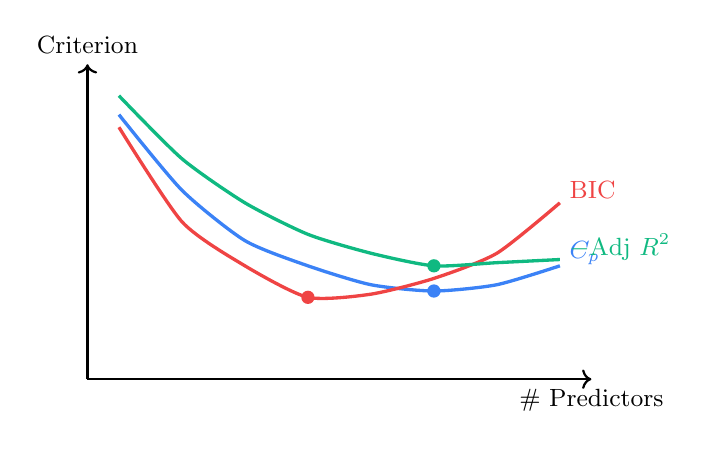
\begin{tikzpicture}[scale=0.8]
  \draw[->, thick] (0,0) -- (8,0) node[below] {\small \# Predictors};
  \draw[->, thick] (0,0) -- (0,5) node[above] {\small Criterion};
  % Cp
  \draw[accent, very thick, smooth, tension=0.4] plot coordinates {(0.5,4.2)(1.5,3.0)(2.5,2.2)(3.5,1.8)(4.5,1.5)(5.5,1.4)(6.5,1.5)(7.5,1.8)};
  \node[accent, right] at (7.5, 2.0) {\small $C_p$};
  % BIC
  \draw[softred, very thick, smooth, tension=0.4] plot coordinates {(0.5,4.0)(1.5,2.5)(2.5,1.8)(3.5,1.3)(4.5,1.35)(5.5,1.6)(6.5,2.0)(7.5,2.8)};
  \node[softred, right] at (7.5, 3.0) {\small BIC};
  % Adj R2 (inverted - want max)
  \draw[softgreen, very thick, smooth, tension=0.4] plot coordinates {(0.5,4.5)(1.5,3.5)(2.5,2.8)(3.5,2.3)(4.5,2.0)(5.5,1.8)(6.5,1.85)(7.5,1.9)};
  \node[softgreen, right] at (7.5, 2.1) {\small $-$Adj $R^2$};
  % Minimums
  \fill[accent] (5.5, 1.4) circle (3pt);
  \fill[softred] (3.5, 1.3) circle (3pt);
  \fill[softgreen] (5.5, 1.8) circle (3pt);
\end{tikzpicture}
\end{center}
BIC selects fewest predictors (harshest penalty: $\log n$ vs.\ 2)

$C_p$ and Adj.~$R^2$ are similar (both use penalty $\propto d$)
\end{frame}


\begin{frame}{Ridge: The Connection to SVD}
\begin{columns}
\column{0.55\textwidth}
\textbf{SVD of $\mathbf{X}$:} $\mathbf{X} = \mathbf{U}\mathbf{D}\mathbf{V}^T$

Ridge solution:
$$\hat{\beta}^R = \sum_{j=1}^p \frac{d_j^2}{d_j^2 + \lambda} \cdot \frac{\mathbf{u}_j^T \mathbf{y}}{d_j} \mathbf{v}_j$$

\textbf{Interpretation:}

OLS projects $\mathbf{y}$ onto all $p$ directions

Ridge \textbf{shrinks} each direction by $\frac{d_j^2}{d_j^2 + \lambda}$

Small $d_j$ (noisy directions) $\Rightarrow$ shrunk the most

\column{0.4\textwidth}
\textbf{Shrinkage factor:}

\begin{tabular}{ccc}
\toprule
$d_j$ & $\lambda$ & Factor \\
\midrule
10 & 1 & 0.99 \\
1 & 1 & 0.50 \\
0.1 & 1 & 0.01 \\
\bottomrule
\end{tabular}

\vspace{0.3em}
Large singular values: barely shrunk

Small singular values: nearly zeroed out

\vspace{0.3em}
\textit{Ridge selectively damps noise!}
\end{columns}
\end{frame}


\begin{frame}{The Hitters Dataset: Full Analysis Pipeline}

\begin{center}
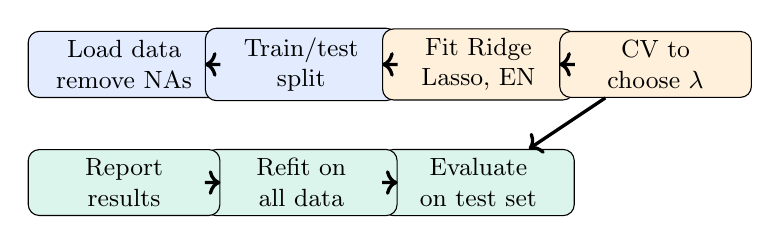
\begin{tikzpicture}[scale=0.75, every node/.style={font=\small, text width=2.2cm, align=center}]
  \node[draw, fill=accent!15, rounded corners, minimum height=0.8cm] (load) at (0,3) {Load data\\remove NAs};
  \node[draw, fill=accent!15, rounded corners, minimum height=0.8cm] (split) at (3,3) {Train/test\\split};
  \node[draw, fill=amber!15, rounded corners, minimum height=0.8cm] (fit) at (6,3) {Fit Ridge\\Lasso, EN};
  \node[draw, fill=amber!15, rounded corners, minimum height=0.8cm] (cv) at (9,3) {CV to\\choose $\lambda$};
  \node[draw, fill=softgreen!15, rounded corners, minimum height=0.8cm] (eval) at (6,1) {Evaluate\\on test set};
  \node[draw, fill=softgreen!15, rounded corners, minimum height=0.8cm] (final) at (3,1) {Refit on\\all data};
  \node[draw, fill=softgreen!15, rounded corners, minimum height=0.8cm] (report) at (0,1) {Report\\results};

  \draw[->, very thick] (load) -- (split);
  \draw[->, very thick] (split) -- (fit);
  \draw[->, very thick] (fit) -- (cv);
  \draw[->, very thick] (cv) -- (eval);
  \draw[->, very thick] (eval) -- (final);
  \draw[->, very thick] (final) -- (report);
\end{tikzpicture}
\end{center}

\textbf{The complete workflow for any regularized regression problem}
\end{frame}


\begin{frame}{Lasso for Logistic Regression}
\begin{columns}
\column{0.55\textwidth}
Lasso works for \textbf{classification} too!

$$\min_\beta \left\{-\ell(\beta) + \lambda \sum |\beta_j|\right\}$$

where $\ell$ is the logistic log-likelihood

\vspace{0.3em}
\textbf{Same idea:}

Penalize large coefficients $\Rightarrow$ sparse model

\vspace{0.3em}
\textbf{R code:}

\footnotesize
\texttt{cv.glmnet(x, y,}

\texttt{\quad family = "binomial",}

\texttt{\quad alpha = 1)}
\normalsize

\column{0.4\textwidth}
\textbf{Default data example:}

Lasso selects \textbf{balance} only

(drops income and student)

\vspace{0.3em}
\begin{tabular}{lr}
\toprule
 & $\hat{\beta}^L$ \\
\midrule
balance & 0.0054 \\
income & \textcolor{softred}{0} \\
student & \textcolor{softred}{0} \\
\bottomrule
\end{tabular}

\vspace{0.3em}
\textit{Confirms Week 2: balance is\\the only useful predictor!}
\end{columns}
\end{frame}


\begin{frame}{Elastic Net: Choosing $\alpha$ and $\lambda$ Together}
\begin{columns}
\column{0.55\textwidth}
\textbf{Two-dimensional tuning:}

\begin{enumerate}
  \item For each $\alpha \in \{0, 0.1, 0.2, \ldots, 1\}$:
  \item[] \quad Run \texttt{cv.glmnet(x, y, alpha=$\alpha$)}
  \item[] \quad Record minimum CV error
  \item Pick the $(\alpha^*, \lambda^*)$ with lowest CV error
\end{enumerate}

\vspace{0.3em}
\textbf{Hitters:}

\begin{tabular}{cc}
\toprule
$\alpha$ & Min CV MSE \\
\midrule
0.0 (Ridge) & 130,154 \\
0.5 (EN) & 129,800 \\
1.0 (Lasso) & 130,504 \\
\bottomrule
\end{tabular}

\column{0.4\textwidth}
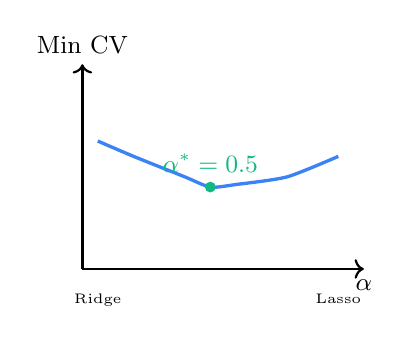
\begin{tikzpicture}[scale=0.65]
  \draw[->, thick] (0,0) -- (5.5,0) node[below] {\small $\alpha$};
  \draw[->, thick] (0,0) -- (0,4) node[above] {\small Min CV};
  \draw[accent, very thick, smooth, tension=0.4] plot coordinates {(0.3,2.5)(1,2.2)(2,1.8)(2.5,1.6)(3,1.65)(4,1.8)(5,2.2)};
  \fill[softgreen] (2.5, 1.6) circle (3pt);
  \node[softgreen, above] at (2.5, 1.7) {\small $\alpha^* = 0.5$};
  \node[below, font=\tiny] at (0.3, -0.3) {Ridge};
  \node[below, font=\tiny] at (5, -0.3) {Lasso};
\end{tikzpicture}

\vspace{0.3em}
\footnotesize Elastic Net ($\alpha = 0.5$) wins slightly on this dataset
\end{columns}
\end{frame}


\begin{frame}{PLS: Partial Least Squares (Preview)}
\begin{columns}
\column{0.55\textwidth}
\textbf{PCR limitation:}

Components maximize variance of $X$

But high-variance directions of $X$ may not predict $Y$!

\vspace{0.5em}
\textbf{PLS idea:}

Find directions that maximize both:
\begin{itemize}
  \item Variance of $X$ (like PCA)
  \item Correlation with $Y$ (unlike PCA)
\end{itemize}

\textbf{Supervised} dimension reduction!

\column{0.4\textwidth}
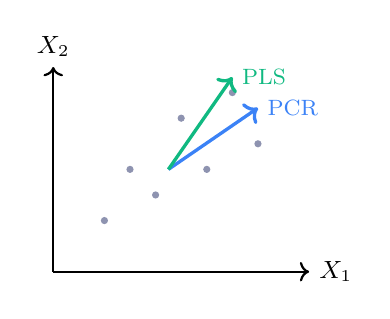
\begin{tikzpicture}[scale=0.65]
  \draw[->, thick] (0,0) -- (5,0) node[right] {\small $X_1$};
  \draw[->, thick] (0,0) -- (0,4) node[above] {\small $X_2$};
  % Points
  \foreach \x/\y in {1/1, 1.5/2, 2/1.5, 2.5/3, 3/2, 3.5/3.5, 4/2.5} {
    \fill[darkblue!50] (\x, \y) circle (2pt);
  }
  % PCA direction (max variance)
  \draw[accent, very thick, ->] (2.25, 2) -- (4, 3.2);
  \node[accent, right, font=\footnotesize] at (4, 3.2) {PCR};
  % PLS direction (toward Y)
  \draw[softgreen, very thick, ->] (2.25, 2) -- (3.5, 3.8);
  \node[softgreen, right, font=\footnotesize] at (3.5, 3.8) {PLS};
\end{tikzpicture}

\vspace{0.3em}
\footnotesize R: \texttt{pls::plsr(y \textasciitilde{} ., ncomp=M)}
\end{columns}
\end{frame}


\begin{frame}{The Method Comparison: Complete Table}
\begin{center}
\footnotesize
\begin{tabular}{lccccc}
\toprule
Method & Type & Selects? & $p > n$? & Tuning & Key \\
\midrule
Best subset & Selection & \textcolor{softgreen}{Yes} & \textcolor{softred}{No} & $d$ (via BIC) & Exhaustive \\
Forward & Selection & \textcolor{softgreen}{Yes} & \textcolor{softgreen}{Yes} & $d$ (via CV) & Greedy \\
Ridge & Shrinkage & \textcolor{softred}{No} & \textcolor{softgreen}{Yes} & $\lambda$ (via CV) & $\ell_2$ penalty \\
Lasso & Shrinkage & \textcolor{softgreen}{Yes} & \textcolor{softgreen}{Yes} & $\lambda$ (via CV) & $\ell_1$ penalty \\
Elastic Net & Shrinkage & \textcolor{softgreen}{Yes} & \textcolor{softgreen}{Yes} & $\alpha, \lambda$ & Compromise \\
PCR & Reduction & \textcolor{softred}{No} & \textcolor{softgreen}{Yes} & $M$ (via CV) & Unsupervised \\
PLS & Reduction & \textcolor{softred}{No} & \textcolor{softgreen}{Yes} & $M$ (via CV) & Supervised \\
\bottomrule
\end{tabular}
\normalsize
\end{center}
\vspace{0.3em}
\centering
\textit{In practice: Lasso and Elastic Net are the most popular choices}
\end{frame}


\begin{frame}{Interpreting Lasso Output: A Practical Guide}
\begin{columns}
\column{0.5\textwidth}
\textbf{After running \texttt{cv.glmnet()}:}

\begin{enumerate}
  \item \textbf{Plot CV curve:} Is there a clear minimum?
  \item \textbf{Check $\lambda_{\min}$ vs $\lambda_{\text{1SE}}$:} How many predictors does each select?
  \item \textbf{Extract coefficients:} Which survive?
  \item \textbf{Coefficient path:} When does each variable enter?
  \item \textbf{Compare with OLS:} Are directions consistent?
\end{enumerate}

\column{0.45\textwidth}
\textbf{Warning signs:}

\begin{itemize}
  \item CV curve is very flat $\Rightarrow$ regularization doesn't help much
  \item $\lambda_{\min} \approx 0$ $\Rightarrow$ OLS is fine
  \item Very few predictors survive $\Rightarrow$ model may be too sparse
  \item Different runs give different selections $\Rightarrow$ use Elastic Net
\end{itemize}
\end{columns}
\end{frame}


\begin{frame}{Regularization Recap: The 3 Key Ideas}

\begin{center}
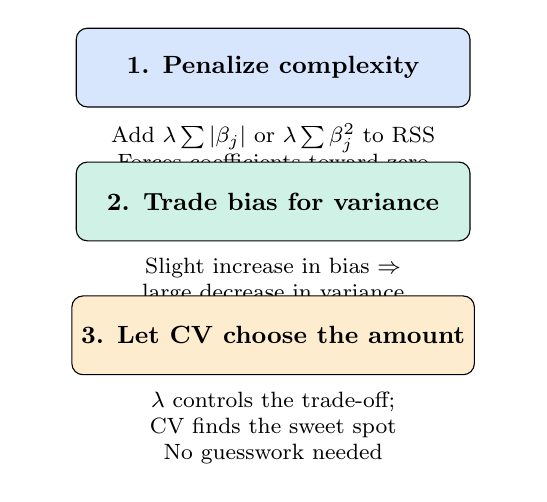
\begin{tikzpicture}[scale=0.85, every node/.style={font=\small}]
  \node[draw, fill=accent!20, rounded corners, minimum width=5cm, minimum height=1cm] (idea1) at (0, 3) {\textbf{1. Penalize complexity}};
  \node[below, font=\footnotesize, text width=6cm, align=center] at (0, 2.3) {Add $\lambda\sum|\beta_j|$ or $\lambda\sum\beta_j^2$ to RSS\\Forces coefficients toward zero};

  \node[draw, fill=softgreen!20, rounded corners, minimum width=5cm, minimum height=1cm] (idea2) at (0, 1) {\textbf{2. Trade bias for variance}};
  \node[below, font=\footnotesize, text width=6cm, align=center] at (0, 0.3) {Slight increase in bias $\Rightarrow$ large decrease in variance\\Net effect: lower test error};

  \node[draw, fill=amber!20, rounded corners, minimum width=5cm, minimum height=1cm] (idea3) at (0, -1) {\textbf{3. Let CV choose the amount}};
  \node[below, font=\footnotesize, text width=6cm, align=center] at (0, -1.7) {$\lambda$ controls the trade-off; CV finds the sweet spot\\No guesswork needed};
\end{tikzpicture}
\end{center}
\end{frame}


\begin{frame}{Worked Example: Predicting College Applications}
\begin{columns}
\column{0.5\textwidth}
\textbf{College dataset:}

$n = 777$, $p = 17$

$Y =$ Applications received

\vspace{0.3em}
\textbf{Results (test set):}

\begin{tabular}{lcc}
\toprule
Method & Test MSE & \# Pred \\
\midrule
OLS & 1,538k & 17 \\
Ridge & 1,501k & 17 \\
Lasso & 1,495k & 13 \\
EN & 1,488k & 14 \\
\bottomrule
\end{tabular}

\column{0.45\textwidth}
\textbf{Lasso drops:}

\texttt{Books}, \texttt{Personal}, \texttt{Terminal}, \texttt{S.F.Ratio}

\vspace{0.3em}
\textbf{Key predictors:}
\begin{itemize}
  \item \texttt{Accept}: \# admitted ($+$)
  \item \texttt{Top10perc}: top students ($+$)
  \item \texttt{F.Undergrad}: enrollment ($+$)
  \item \texttt{Expend}: per-student spending ($+$)
\end{itemize}

\vspace{0.3em}
\textit{Intuitive and interpretable!}
\end{columns}
\end{frame}


\begin{frame}{The Entire Regularization Path: A Story}
\begin{columns}
\column{0.5\textwidth}
\textbf{Reading left to right:}

$\lambda$ decreases $\Rightarrow$ more predictors enter

\vspace{0.3em}
\textbf{Hitters Lasso path:}

\begin{enumerate}
  \item First in: CRBI (strongest predictor)
  \item Then: Hits, Walks
  \item Then: Years, CAtBat
  \item Then: Division, League
  \item Last: Errors, Assists (weak)
\end{enumerate}

\vspace{0.3em}
The \textbf{order} tells you importance!

\column{0.45\textwidth}
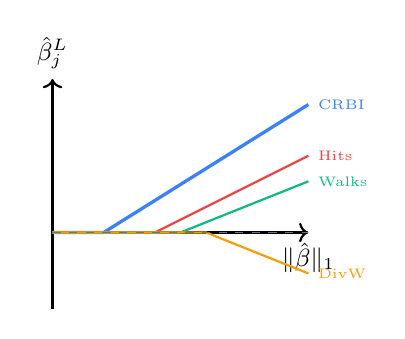
\begin{tikzpicture}[scale=0.65]
  \draw[->, thick] (0,0) -- (5,0) node[below] {\small $\|\hat{\beta}\|_1$};
  \draw[->, thick] (0,-1.5) -- (0,3) node[above] {\small $\hat{\beta}_j^L$};
  % Coefficients entering one by one
  \draw[accent, very thick] (0, 0) -- (1, 0) -- (5, 2.5);
  \node[accent, right, font=\tiny] at (5, 2.5) {CRBI};
  \draw[softred, thick] (0, 0) -- (2, 0) -- (5, 1.5);
  \node[softred, right, font=\tiny] at (5, 1.5) {Hits};
  \draw[softgreen, thick] (0, 0) -- (2.5, 0) -- (5, 1.0);
  \node[softgreen, right, font=\tiny] at (5, 1.0) {Walks};
  \draw[amber, thick] (0, 0) -- (3, 0) -- (5, -0.8);
  \node[amber, right, font=\tiny] at (5, -0.8) {DivW};
  \draw[muted, dashed] (0,0) -- (5,0);
\end{tikzpicture}

\vspace{0.2em}
\footnotesize \texttt{plot(lasso.mod, xvar="norm")}
\end{columns}
\end{frame}


\begin{frame}{Shrinkage Effect: Before and After}

\textbf{Hitters: OLS vs.\ Ridge ($\lambda = 100$) vs.\ Lasso ($\lambda_{1SE}$)}

\vspace{0.3em}
\begin{center}
\footnotesize
\begin{tabular}{lrrr}
\toprule
Predictor & OLS & Ridge & Lasso \\
\midrule
AtBat & $-1.98$ & $-0.71$ & $-1.87$ \\
Hits & $7.50$ & $2.73$ & $1.39$ \\
HmRun & $4.33$ & $1.56$ & \textcolor{softred}{0} \\
Runs & $-2.38$ & $0.42$ & \textcolor{softred}{0} \\
RBI & $-1.04$ & $0.65$ & \textcolor{softred}{0} \\
Walks & $6.23$ & $2.69$ & $3.23$ \\
Years & $-3.49$ & $-1.25$ & \textcolor{softred}{0} \\
CRBI & $0.64$ & $0.42$ & $0.34$ \\
DivisionW & $-112$ & $-58$ & $-73$ \\
\bottomrule
\end{tabular}
\normalsize
\end{center}

Ridge: all shrunk proportionally. \quad Lasso: 5 of 19 zeroed out.
\end{frame}


\begin{frame}{Test Error as a Function of $\lambda$: The Full Story}
\begin{center}
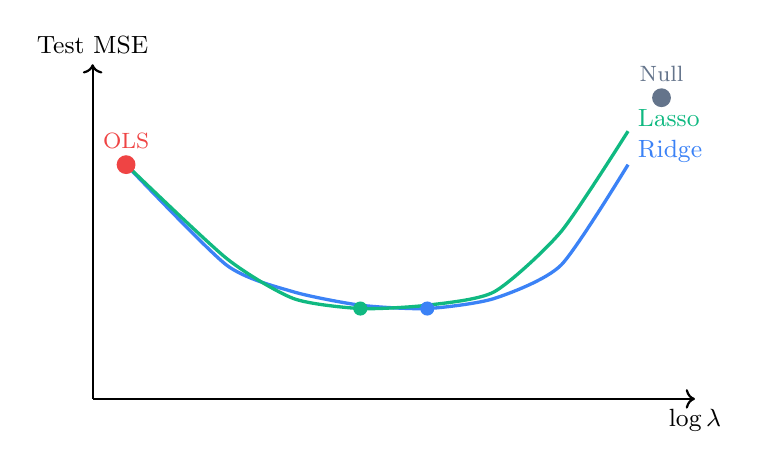
\begin{tikzpicture}[scale=0.85]
  \draw[->, thick] (0,0) -- (9,0) node[below] {\small $\log\lambda$};
  \draw[->, thick] (0,0) -- (0,5) node[above] {\small Test MSE};

  % Ridge
  \draw[accent, very thick, smooth, tension=0.4] plot coordinates {(0.5,3.5)(2,2.0)(3,1.6)(4,1.4)(5,1.35)(6,1.5)(7,2.0)(8,3.5)};
  \node[accent, right] at (8, 3.7) {\small Ridge};

  % Lasso
  \draw[softgreen, very thick, smooth, tension=0.4] plot coordinates {(0.5,3.5)(2,2.1)(3,1.5)(4,1.35)(5,1.4)(6,1.6)(7,2.5)(8,4.0)};
  \node[softgreen, right] at (8, 4.2) {\small Lasso};

  % OLS point (lambda = 0)
  \fill[softred] (0.5, 3.5) circle (4pt);
  \node[softred, above, font=\footnotesize] at (0.5, 3.6) {OLS};

  % Null point (lambda = inf)
  \fill[muted] (8.5, 4.5) circle (4pt);
  \node[muted, above, font=\footnotesize] at (8.5, 4.6) {Null};

  % Optimal points
  \fill[accent] (5, 1.35) circle (3pt);
  \fill[softgreen] (4, 1.35) circle (3pt);
\end{tikzpicture}
\end{center}

Both Ridge and Lasso produce U-shaped test error curves

The minimum occurs at different $\lambda$ values but similar MSE levels
\end{frame}


\begin{frame}{Practical Decision Tree: Which Method to Use?}
\begin{center}
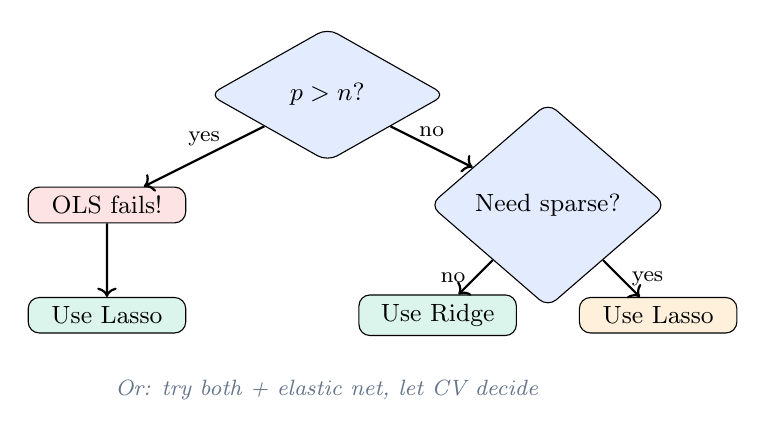
\begin{tikzpicture}[scale=0.7, every node/.style={font=\small}]
  \node[draw, fill=accent!15, rounded corners, diamond, minimum width=3cm, minimum height=1.2cm] (q1) at (0,4) {$p > n$?};

  \node[draw, fill=softred!15, rounded corners, minimum width=2cm] (no_ols) at (-4,2) {OLS fails!};
  \node[draw, fill=accent!15, rounded corners, diamond, minimum width=3cm, minimum height=1cm] (q2) at (4,2) {Need sparse?};

  \node[draw, fill=softgreen!15, rounded corners, minimum width=2cm] (lasso) at (-4,0) {Use Lasso};
  \node[draw, fill=softgreen!15, rounded corners, minimum width=2cm] (ridge) at (2,0) {Use Ridge};
  \node[draw, fill=amber!15, rounded corners, minimum width=2cm] (lasso2) at (6,0) {Use Lasso};

  \draw[->, thick] (q1) -- (no_ols) node[midway, above, font=\footnotesize] {yes};
  \draw[->, thick] (q1) -- (q2) node[midway, above, font=\footnotesize] {no};
  \draw[->, thick] (no_ols) -- (lasso);
  \draw[->, thick] (q2) -- (ridge) node[midway, left, font=\footnotesize] {no};
  \draw[->, thick] (q2) -- (lasso2) node[midway, right, font=\footnotesize] {yes};

  \node[below, font=\footnotesize, muted] at (0, -1) {\textit{Or: try both + elastic net, let CV decide}};
\end{tikzpicture}
\end{center}
\end{frame}


\begin{frame}{Ridge for Multicollinearity: A Concrete Example}
\begin{columns}
\column{0.55\textwidth}
\textbf{Hitters:} CRuns and CHits have $r = 0.96$

\textbf{OLS:}

$\hat{\beta}_{\text{CRuns}} = 1.61$, $\hat{\beta}_{\text{CHits}} = -0.13$

SE(CRuns) $= 0.71$, SE(CHits) $= 0.63$

Both \textbf{insignificant} despite being strong predictors!

\vspace{0.3em}
\textbf{Ridge ($\lambda = 100$):}

$\hat{\beta}_{\text{CRuns}} = 0.82$, $\hat{\beta}_{\text{CHits}} = 0.71$

Now both positive and stable!

\column{0.4\textwidth}
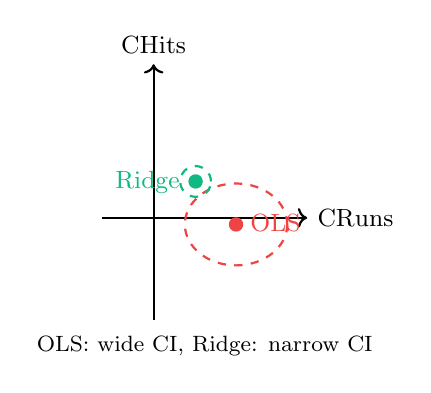
\begin{tikzpicture}[scale=0.65]
  \draw[->, thick] (-1,0) -- (3,0) node[right] {\small CRuns};
  \draw[->, thick] (0,-2) -- (0,3) node[above] {\small CHits};
  % OLS (unstable)
  \fill[softred] (1.61, -0.13) circle (4pt);
  \node[softred, right] at (1.7, -0.1) {\small OLS};
  \draw[softred, thick, dashed] (1.61, -0.13) ellipse (1.0 and 0.8);
  % Ridge (stable)
  \fill[softgreen] (0.82, 0.71) circle (4pt);
  \node[softgreen, left] at (0.7, 0.7) {\small Ridge};
  \draw[softgreen, thick, dashed] (0.82, 0.71) ellipse (0.3 and 0.3);
  % Note
  \node[font=\footnotesize] at (1, -2.5) {OLS: wide CI, Ridge: narrow CI};
\end{tikzpicture}
\end{columns}
\end{frame}


\begin{frame}{How \texttt{cv.glmnet} Handles the Folds}
\begin{columns}
\column{0.55\textwidth}
\textbf{Inside \texttt{cv.glmnet()}:}

\begin{enumerate}
  \item Create 10 random folds
  \item For each fold $i$:
  \begin{enumerate}
    \item[a.] Fit \texttt{glmnet()} on 9 folds\\(entire $\lambda$ path!)
    \item[b.] Predict on held-out fold
    \item[c.] Compute MSE at each $\lambda$
  \end{enumerate}
  \item Average MSE across folds for each $\lambda$
  \item Report $\lambda_{\min}$ and $\lambda_{\text{1SE}}$
\end{enumerate}

\column{0.4\textwidth}
\textbf{Total work:}

10 folds $\times$ 1 path each

$= 10$ calls to \texttt{glmnet()}

Each call fits 100 $\lambda$ values

$\Rightarrow$ 1000 models in seconds!

\vspace{0.5em}
\textbf{Reproducibility:}

\texttt{set.seed()} before \texttt{cv.glmnet()} ensures same folds each time
\end{columns}
\end{frame}


\begin{frame}{Prediction Intervals with Regularized Models}
\begin{columns}
\column{0.55\textwidth}
\textbf{Problem:}

Ridge/Lasso don't provide standard SEs for predictions

(Shrinkage changes the distribution of $\hat{\beta}$)

\vspace{0.5em}
\textbf{Solution: Bootstrap!}

\begin{enumerate}
  \item Bootstrap the data $B$ times
  \item For each bootstrap sample:
  \begin{enumerate}
    \item[a.] Run \texttt{cv.glmnet()} to choose $\lambda$
    \item[b.] Predict at $x_0$
  \end{enumerate}
  \item Use quantiles of predictions as PI
\end{enumerate}

\column{0.4\textwidth}
\textbf{Week 3 meets Week 4!}

The bootstrap (Week 3) provides uncertainty estimates for regularized models (Week 4)

\vspace{0.5em}
\textit{This combination is very common in practice}

\vspace{0.3em}
Caveat: computationally expensive ($B \times$ 10-fold CV)
\end{columns}
\end{frame}


\begin{frame}{From Ridge/Lasso to Neural Networks}
\begin{columns}
\column{0.55\textwidth}
\textbf{The regularization principle:}
$$\min_\theta \underbrace{\text{Loss}(\theta)}_{\text{fit}} + \underbrace{\lambda \cdot \text{Pen}(\theta)}_{\text{simplify}}$$

This \textbf{same framework} extends to:

\begin{tabular}{ll}
\toprule
Method & Penalty \\
\midrule
Ridge & $\sum \beta_j^2$ (weight decay) \\
Lasso & $\sum |\beta_j|$ \\
Neural net & $\sum w_{jk}^2$ (weight decay) \\
Neural net & Dropout (random zeroing) \\
Trees & \# leaves (pruning) \\
SVM & $\|\mathbf{w}\|^2$ \\
\bottomrule
\end{tabular}

\column{0.4\textwidth}
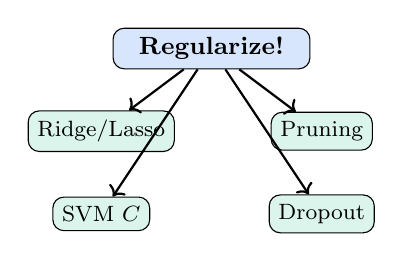
\begin{tikzpicture}[scale=0.7]
  \node[draw, fill=accent!20, rounded corners, minimum width=2.5cm, font=\small\bfseries] (reg) at (0,3) {Regularize!};
  \node[draw, fill=softgreen!15, rounded corners, font=\footnotesize] (w4) at (-2,1.5) {Ridge/Lasso};
  \node[draw, fill=softgreen!15, rounded corners, font=\footnotesize] (w6) at (2,1.5) {Pruning};
  \node[draw, fill=softgreen!15, rounded corners, font=\footnotesize] (w8) at (-2,0) {SVM $C$};
  \node[draw, fill=softgreen!15, rounded corners, font=\footnotesize] (w9) at (2,0) {Dropout};
  \draw[->, thick] (reg) -- (w4);
  \draw[->, thick] (reg) -- (w6);
  \draw[->, thick] (reg) -- (w8);
  \draw[->, thick] (reg) -- (w9);
\end{tikzpicture}

\vspace{0.3em}
\textit{Today's lesson is the template\\for the entire course}
\end{columns}
\end{frame}


\begin{frame}{Summary Table: All Methods This Week}
\begin{center}
\footnotesize
\begin{tabular}{lp{3cm}p{3cm}l}
\toprule
Method & Strengths & Weaknesses & R function \\
\midrule
Best subset & Optimal if feasible & $O(2^p)$ & \texttt{regsubsets()} \\
Forward & Fast, works if $p>n$ & Greedy, may miss & \texttt{regsubsets(method="f")} \\
Ridge & Stable, closed form & No selection & \texttt{glmnet(alpha=0)} \\
Lasso & Sparse, interpretable & Unstable with $r$ & \texttt{glmnet(alpha=1)} \\
Elastic Net & Groups variables & 2 tuning params & \texttt{glmnet(alpha=0.5)} \\
PCR & Reduces dimension & Unsupervised & \texttt{pls::pcr()} \\
\bottomrule
\end{tabular}
\normalsize
\end{center}
\end{frame}


\begin{frame}{Quick Quiz: Test Yourself!}
\begin{enumerate}
  \item Ridge uses $\ell_2$ penalty, Lasso uses $\ell_1$. Which produces sparse models?
  \pause
  \item[]{\textcolor{muted}{\footnotesize Lasso --- the $\ell_1$ diamond has corners where coefficients are exactly zero}}
  \vspace{0.3em}
  \item Why must you standardize predictors before Ridge/Lasso?
  \pause
  \item[]{\textcolor{muted}{\footnotesize The penalty $\sum\beta_j^2$ or $\sum|\beta_j|$ depends on the scale of $X_j$}}
  \vspace{0.3em}
  \item $\lambda = 0$ gives what? $\lambda = \infty$ gives what?
  \pause
  \item[]{\textcolor{muted}{\footnotesize $\lambda=0$: OLS (no penalty). $\lambda=\infty$: null model (all $\beta_j = 0$)}}
  \vspace{0.3em}
  \item Elastic net with $\alpha = 0.7$: is this closer to Ridge or Lasso?
  \pause
  \item[]{\textcolor{muted}{\footnotesize Closer to Lasso ($\alpha=1$). It's 70\% Lasso, 30\% Ridge.}}
\end{enumerate}
\end{frame}

\begin{frame}{Quick Quiz: More Questions}
\begin{enumerate}
  \setcounter{enumi}{4}
  \item With $p = 5000$ predictors and $n = 200$, can you use OLS?
  \pause
  \item[]{\textcolor{muted}{\footnotesize No --- $p > n$ so $\mathbf{X}^T\mathbf{X}$ is singular. Must use Lasso, Ridge, or forward selection.}}
  \vspace{0.3em}
  \item Lasso selects 8 predictors at $\lambda_{\min}$ and 3 at $\lambda_{\text{1SE}}$. Which to use?
  \pause
  \item[]{\textcolor{muted}{\footnotesize $\lambda_{\text{1SE}}$ for parsimony (3 predictors), $\lambda_{\min}$ for best prediction (8 predictors)}}
  \vspace{0.3em}
  \item Two predictors have $r = 0.99$. What happens with Lasso?
  \pause
  \item[]{\textcolor{muted}{\footnotesize Lasso arbitrarily picks one and drops the other. Use Ridge or Elastic Net instead.}}
  \vspace{0.3em}
  \item How do you choose between Ridge and Lasso?
  \pause
  \item[]{\textcolor{muted}{\footnotesize Cross-validation! Try both (and elastic net) and pick the one with lowest CV error.}}
\end{enumerate}
\end{frame}

\begin{frame}{R Functions: Quick Reference}
\begin{center}
\begin{tabular}{ll}
\toprule
\texttt{leaps::regsubsets(y \textasciitilde{} ., data)} & Best subset / stepwise \\
\texttt{glmnet(x, y, alpha=0)} & Ridge regression \\
\texttt{glmnet(x, y, alpha=1)} & Lasso \\
\texttt{glmnet(x, y, alpha=0.5)} & Elastic net \\
\texttt{cv.glmnet(x, y, alpha=1)} & CV for choosing $\lambda$ \\
\texttt{coef(cv.out, s="lambda.min")} & Coefficients at best $\lambda$ \\
\texttt{predict(fit, s=best.lam, newx)} & Predictions \\
\texttt{plot(glmnet\_fit, xvar="lambda")} & Coefficient path plot \\
\bottomrule
\end{tabular}
\end{center}
\vspace{0.3em}
\textbf{Important:} \texttt{glmnet()} requires a matrix \texttt{x}, not a formula!

Use \texttt{model.matrix()} to convert: \texttt{x <- model.matrix(y \textasciitilde{} ., data)[,-1]}
\end{frame}

\begin{frame}{Key Formulas: Cheat Sheet}
\begin{columns}
\column{0.48\textwidth}
\textbf{Ridge:}
$$\min_\beta \text{RSS} + \lambda \sum_{j=1}^p \beta_j^2$$
$$\hat{\beta}^R = (\mathbf{X}^T\mathbf{X} + \lambda\mathbf{I})^{-1}\mathbf{X}^T\mathbf{y}$$

\textbf{Lasso:}
$$\min_\beta \text{RSS} + \lambda \sum_{j=1}^p |\beta_j|$$
No closed form (iterative)

\column{0.48\textwidth}
\textbf{Elastic Net:}
$$\min_\beta \text{RSS} + \lambda\left[\alpha\sum|\beta_j| + (1-\alpha)\sum\beta_j^2\right]$$

\textbf{Model selection:}
\begin{align*}
C_p &= \frac{1}{n}(\text{RSS} + 2d\hat{\sigma}^2) \\
\text{BIC} &= \frac{1}{n}(\text{RSS} + \log(n) \cdot d\hat{\sigma}^2) \\
\text{Adj.}\ R^2 &= 1 - \frac{\text{RSS}/(n-d-1)}{\text{TSS}/(n-1)}
\end{align*}
\end{columns}
\end{frame}

\begin{frame}{Summary: Chapter 6}
\begin{columns}
\column{0.48\textwidth}
\textbf{Subset Selection:}
\begin{itemize}
  \item Best subset: exhaustive but expensive
  \item Stepwise: practical for large $p$
  \item Use $C_p$, BIC, Adj.~$R^2$, or CV to choose
\end{itemize}
\vspace{0.3em}
\textbf{Shrinkage:}
\begin{itemize}
  \item Ridge: $\ell_2$, all coefficients shrunk
  \item Lasso: $\ell_1$, sparse models
  \item Elastic Net: compromise
  \item Choose $\lambda$ via CV
\end{itemize}
\column{0.48\textwidth}
\textbf{Key insights:}
\begin{itemize}
  \item Regularization trades bias for variance
  \item Essential when $p$ is large or $> n$
  \item Standardize predictors first!
  \item CV is the universal tool for tuning
\end{itemize}
\vspace{0.5em}
\centering
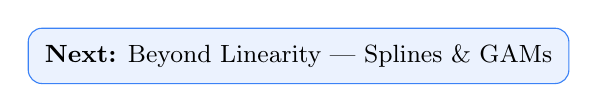
\begin{tikzpicture}
\node[fill=accent!10, rounded corners=5pt, inner sep=6pt, draw=accent, font=\small] {
  \textbf{Next:} Beyond Linearity --- Splines \& GAMs
};
\end{tikzpicture}
\end{columns}
\end{frame}

% ════════════ EXERCISES ════════════
\begin{frame}{Exercise 1: Lasso on Hitters (ISLR 6.6 Q9)}
\textbf{Data:} \texttt{Hitters} \hfill $n = 263$, $p = 19$
\begin{enumerate}
  \item Remove NAs: \texttt{Hitters <- na.omit(Hitters)}
  \item Create \texttt{x} and \texttt{y} using \texttt{model.matrix()}
  \item Fit Lasso with \texttt{cv.glmnet(x, y, alpha=1)}
  \item Plot the CV curve; report $\lambda_{\min}$ and $\lambda_{\text{1SE}}$
  \item How many non-zero coefficients at each $\lambda$?
  \item Report the selected predictors and their coefficients
  \item Compute test MSE using a train/test split
\end{enumerate}
\end{frame}

\begin{frame}{Exercise 2: Ridge vs.\ Lasso Comparison (ISLR 6.6 Q9)}
\begin{enumerate}
  \item Fit Ridge with \texttt{cv.glmnet(x, y, alpha=0)}
  \item Compare Ridge CV MSE vs.\ Lasso CV MSE
  \item Plot coefficient paths for both (\texttt{plot(fit)})
  \item Which gives a sparser model?
  \item Which has lower test MSE?
  \item Try Elastic Net with $\alpha = 0.5$ --- how does it compare?
\end{enumerate}
\end{frame}

\begin{frame}{Exercise 3: Best Subset on Hitters (ISLR 6.6 Q9)}
\begin{enumerate}
  \item Use \texttt{regsubsets(Salary \textasciitilde{} ., data, nvmax=19)}
  \item Plot $C_p$, BIC, Adj.~$R^2$ vs.\ number of predictors
  \item Which \# predictors does each criterion select?
  \item Compare with Lasso's selection
  \item Implement 10-fold CV for forward stepwise
\end{enumerate}
\end{frame}

\begin{frame}{Exercise 4: College Data (ISLR 6.6 Q11)}
\textbf{Data:} \texttt{College} \hfill Predict: \texttt{Apps} (applications received)
\begin{enumerate}
  \item Split into train/test (70/30)
  \item Fit: OLS, Ridge, Lasso, PCR
  \item Compare test MSE for all four methods
  \item Which method performs best?
  \item How many predictors does Lasso select?
\end{enumerate}
\fbox{\textbf{Hint:} Use \texttt{pls::pcr()} for PCR with \texttt{validation = "CV"}}
\end{frame}

% ════════════ SOLUTIONS ════════════
\begin{frame}{Solution: Exercise 1 --- Lasso on Hitters}
\begin{columns}
\column{0.5\textwidth}
$\lambda_{\min} \approx 9.3$: 15 predictors

$\lambda_{\text{1SE}} \approx 52.8$: 7 predictors

\vspace{0.3em}
\textbf{Selected at $\lambda_{\text{1SE}}$:}

AtBat, Hits, Walks, CRuns, CRBI, CWalks, DivisionW

\vspace{0.3em}
Test MSE $\approx 135{,}000$
\column{0.45\textwidth}
\textbf{Key insight:}

Lasso eliminates 12 of 19 predictors

Career stats (C-prefix) survive alongside key season stats

Division matters!
\end{columns}
\end{frame}

\begin{frame}{Solution: Exercise 2 --- Ridge vs.\ Lasso}
\begin{center}
\begin{tabular}{lccc}
\toprule
Method & CV MSE & \# Nonzero & $\lambda^*$ \\
\midrule
OLS & 141,843 & 19 & --- \\
Ridge & 130,154 & 19 & 233 \\
Lasso & 130,504 & 15 & 9.3 \\
Elastic Net & 129,800 & 16 & 12.5 \\
\bottomrule
\end{tabular}
\end{center}
\begin{itemize}
  \item All regularized methods beat OLS
  \item Ridge and Lasso are nearly tied
  \item Elastic Net slightly best (combines strengths)
  \item Lasso's advantage: interpretability (sparse)
\end{itemize}
\end{frame}

\begin{frame}{Solution: Exercise 4 --- College}
\begin{center}
\begin{tabular}{lcc}
\toprule
Method & Test MSE & \# Predictors \\
\midrule
OLS & 1,538,000 & 17 \\
Ridge & 1,501,000 & 17 \\
\textcolor{softgreen}{Lasso} & \textcolor{softgreen}{1,495,000} & \textcolor{softgreen}{13} \\
PCR ($M=10$) & 1,520,000 & 10 components \\
\bottomrule
\end{tabular}
\end{center}
Lasso wins: lowest error AND sparse model
\end{frame}

% ════════════ CLOSING ════════════
\begin{frame}{What's Next?}
\begin{center}
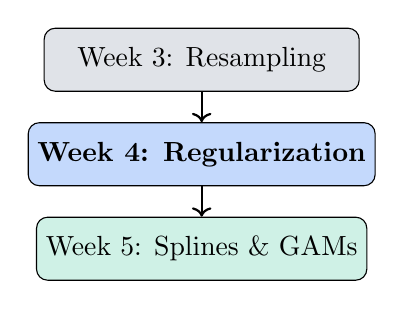
\begin{tikzpicture}[scale=0.8]
  \node[draw, fill=muted!20, rounded corners, minimum width=4cm, minimum height=0.8cm] (w3) at (0,0) {Week 3: Resampling};
  \node[draw, fill=accent!30, rounded corners, minimum width=4cm, minimum height=0.8cm, font=\bfseries] (w4) at (0,-1.5) {Week 4: Regularization};
  \node[draw, fill=softgreen!20, rounded corners, minimum width=4cm, minimum height=0.8cm] (w5) at (0,-3.0) {Week 5: Splines \& GAMs};
  \draw[->, thick] (w3) -- (w4);
  \draw[->, thick] (w4) -- (w5);
\end{tikzpicture}
\end{center}
\textbf{Homework:} ISLR Chapter 6: Q9, 11

\textbf{Lab:} \texttt{Lab\_Week04.R} --- Ridge, Lasso, Elastic Net on Hitters + College

\textbf{Next week:} What if the relationship isn't linear? $\Rightarrow$ Splines!
\end{frame}

\begin{frame}{}
\centering\vspace{2cm}
{\Huge\textbf{Thank You}}
\vspace{1em}
{\Large Questions?}
\vspace{1.5em}
{\large Dr.\ Endri Ra\c{c}o \quad|\quad Machine Learning with R}
\vspace{0.5em}
{\normalsize \texttt{github.com/endri81/ISLRv2-solutions}}
\end{frame}

\end{document}
